%____________________________________________________________________________||
\section{Interpretation in Dark Matter models} \label{sec:darkmatter}

In Run~1, the results of the \alphat analysis were interpreted in the context of
supersymmetric simplified models. For Run~2, significant effort has been invested
in extending the analysis strategy to include searches for the production of dark
matter, namely the inclusion of the asymmetric and monojet categories.

The generic signature of dark matter pair production in colliders is missing
transverse momentum from the dark matter along with recoiling energetic visible
particles that are used to trigger the event. First analyses used contact 
operators~\cite{Goodman:2010ku} in effective field theories (EFTs) with various 
coupling structures to interpret dark matter searches. Experimental limits using
monojet final states have been published using 7 and 8 TeV LHC 
data~\cite{Chatrchyan:2012me,ATLAS:2012ky} for a variety of operators.


The lack of predictive information and severe validity constraints of EFTs have
led to the development of minimal simplified dark matter (MSDM) models.
These models enable the comparison between different experimental
searches in a relatively model-independent way~\cite{Buchmueller:2014yoa}.


The \alphat analysis is sensitive to DM production in association with both
light ($g,~u,~d,~c,~s$) and heavy flavoured ($b,~t$) jets. In this section we
present the expected sensitivity of the analysis to these topologies with 12.9~\ifb
of 13 TeV data. The simplified models considered in the interpretations are those
recommended by the ATLAS-CMS DM Forum for early LHC Run~2 searches. We have
utilised all available Spring15 samples of the corresponding models that were
available at the time of writing. These samples populate key regions of the
{\mphi-\mchi} mass plane, and correspond roughly to those shown in
Tab.~\ref{tab:DMgrid}.

\begin{table}[h!] \centering \begin{tabular}{l|llllllllll} \hline \hline
\mchi & \multicolumn{10}{c}{\mphi} \\
\hline
1    & 10 & 20 & 50 & 100 & 200 & 300 & 500 & 1000 & 2000 & 10000 \\
10   & 10 & 15 & 50 & 100 &     &     &     &      &      & 10000 \\
50   & 10 &    & 50 & 95  & 200 & 300 &     &      &      & 10000 \\
150  & 10 &    &    &     & 200 & 295 & 500 & 1000 &      & 10000 \\ 
500  & 10 &    &    &     &     &     & 500 & 995  &      & 10000 \\
1000 & 10 &    &    &     &     &     &     & 1000 & 1995 & 10000 \\
\hline \hline \end{tabular}
\caption{Benchmark dark matter and mediator masses. The parameter space follows
the DM Forum recommendations~\cite{Abercrombie:2015wmb}. Points are chosen 
roughly equidistant on a logarithmic scale. Points on the on-shell diagonal are
always chosen to be 5 GeV away from the threshold to avoid numerical
instabilities in the event generation.} \label{tab:DMgrid} \end{table}


\subsection{Simplified Dark Matter models} \label{sec:dm_smdm}

The light flavour simplified models consist of a DM particle \pchi of mass
\mchi that is a Dirac fermion, and a spin-1 (vector or axial-vector) or spin-0
(scalar or pseudoscalar) mediating particle \pphi of mass \mphi in an
$s$-channel. The heavy flavour simplified models are similar to light flavour
models; however, the production of the mediator is associated with a \ttNew
or \bbNew pair. The couplings of the mediator with the standard model and dark
matter particles are given by \gsm and \gdm, respectively. The recommendations
by the DM Forum on the choice of couplings is $\gsm=1$, $\gdm=1$ for
(pseudo)scalar models, and $\gsm=0.25$, $\gdm=1$ for (axial-)vector models.
Assuming that no additional visible or invisible particles contribute to the decay 
of the mediator, we impose the minimal width determined by the choice of couplings. 
Examples of Feynman diagrams are shown in Fig.~\ref{fig:DMfeynman} and 
\ref{fig:feynman_hf}.

\begin{figure}[h!] \centering
  \subfigure{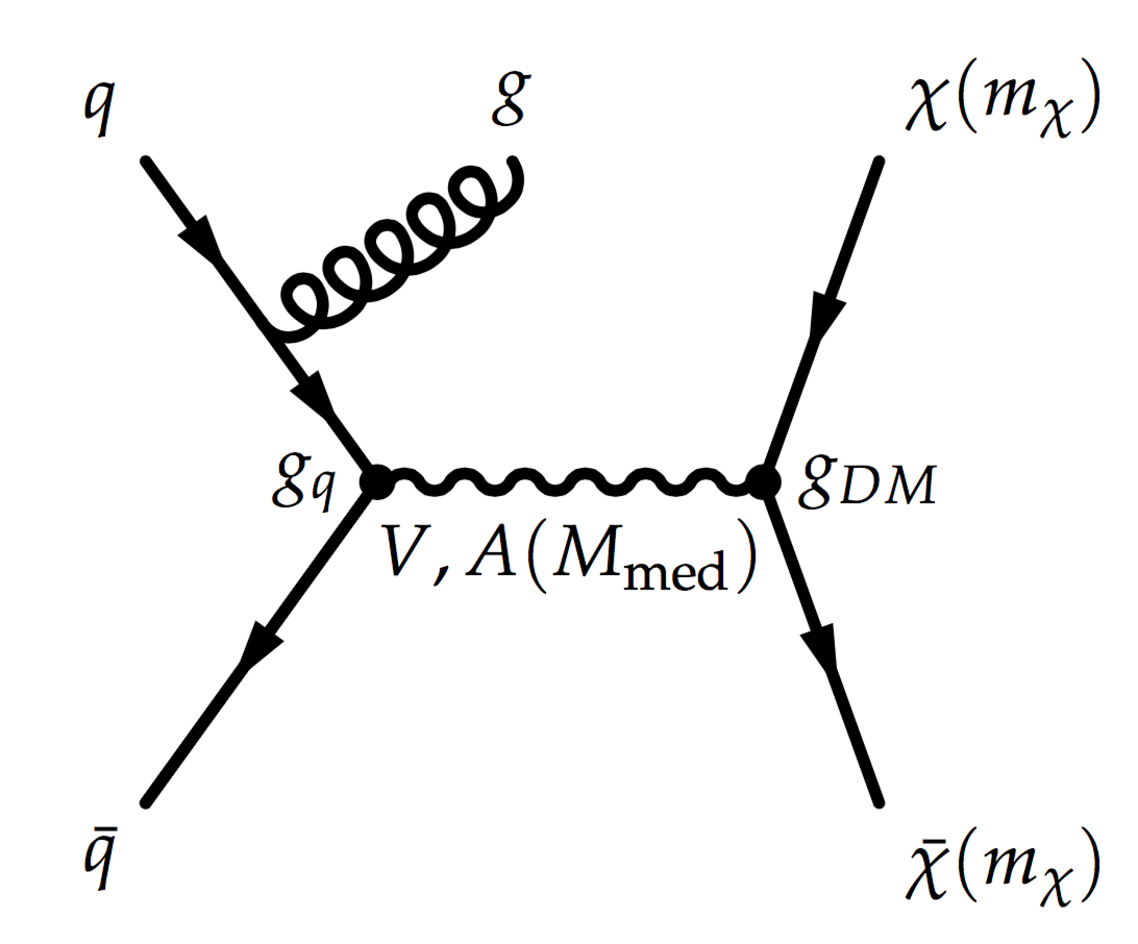
\includegraphics[width=0.35\textwidth]{figures/DMplots/feynman_light_jet.pdf}}
  \caption{Feynman diagram of DM pair production in light jet hadronic final states. \cite{Abercrombie:2015wmb}}
  \label{fig:DMfeynman} 
\end{figure}

\begin{figure}[h!] \centering
  \subfigure{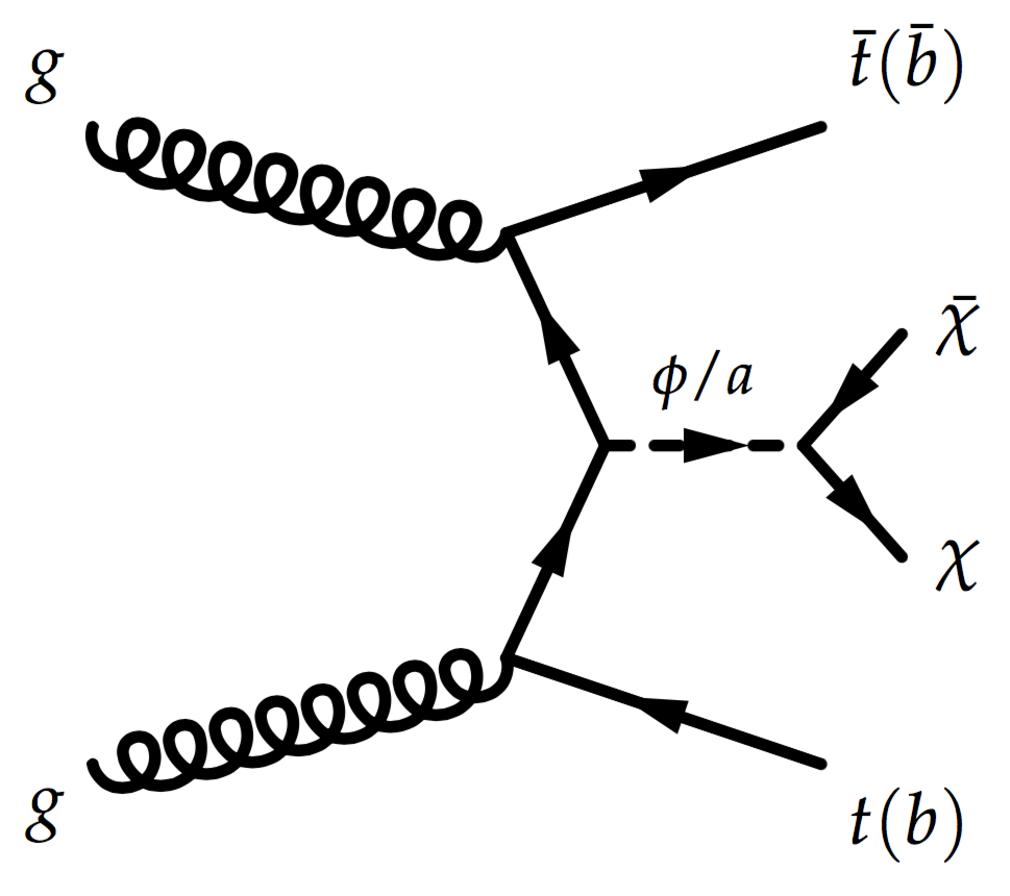
\includegraphics[width=0.35\textwidth]{figures/DMplots/feynman_hf.pdf}}
  \caption{Feynman diagram of the pair production of Dark Matter particles in
  association with $t\bar{t}$ or $b\bar{b}$. \cite{Abercrombie:2015wmb}}
  \label{fig:feynman_hf}
\end{figure}

%Assuming 2~\ifb of data we list the cross sections, yields and selection  efficiencies for the four light jet models in Tables~\ref{summaryTableAN_DMV_xs10_g0p25_2p1fb_exp}-\ref{summaryTableAN_DMS_xs10_g1p0_2p1fb_exp}. 
The signal selection efficiencies are around $\sim 1$\% for mass points near the expected exclusion
region, and are correspondingly larger (smaller) for higher (lower) mass points.
The asymmetric and monojet categories are seen to almost double the acceptance
to these models compared to the Run~1 symmetric categories alone, justifying the
inclusion of these selections into the analysis.

The list of simplified DM MC samples, along with the number of events 
generated, are shown in Tab.~\ref{tab:dmj_av}-\ref{tab:dmtt_s}, respectively.

%\begin{table}[]
%    \centering
%    \begin{tabular}{lrrr}
%        \hline\hline
%        Sample & \mphi & \mchi & NGen \\
%        \hline
%        DM+jets S &   10 &   1 & 296800 \\
%        DM+jets S &  100 &   1 & 293600 \\
%        DM+jets S &  100 &  50 & 297000 \\
%        DM+jets S &  300 &   1 &  50000 \\
%        DM+jets S &  300 & 100 & 292600 \\
%        DM+jets S &  500 &   1 & 294800 \\
%        DM+jets S &  500 & 150 & 298800 \\
%        DM+jets S & 1000 &   1 & 300000 \\
%        DM+jets S & 1250 &   1 & 297200 \\
%        DM+jets S & 1250 &  10 & 289200 \\
%        DM+jets S & 1250 &  50 & 295800 \\
%        DM+jets S & 1250 & 200 & 296000 \\
%        DM+jets S & 1250 & 250 & 294000 \\
%        DM+jets S & 1250 & 300 & 290800 \\
%        DM+jets S & 1250 & 350 & 292800 \\
%        DM+jets S & 1250 & 400 & 283800 \\
%        DM+jets S & 1500 &   1 & 295400 \\
%        DM+jets S & 1500 &  10 & 288000 \\
%        DM+jets S & 1500 &  50 & 293600 \\
%        DM+jets S & 1500 & 100 & 287200 \\
%        DM+jets S & 1500 & 200 & 294200 \\
%        DM+jets S & 1500 & 250 & 286600 \\
%        DM+jets S & 1500 & 300 & 295600 \\
%        DM+jets S & 1500 & 350 & 299600 \\
%        DM+jets S & 1500 & 400 & 300000 \\
%        DM+jets S & 2000 &   1 &  50000 \\
%        \hline\hline
%    \end{tabular}
%    \caption{DM+jets signal simulations using scalar (S) couplings. The last number gives the number of events generated.}
%    \label{tab:dmj_s}
%\end{table}

%\begin{table}[]
%    \centering
%    \begin{tabular}{lrrr}
%        \hline\hline
%        Sample & \mphi & \mchi & NGen \\
%        \hline  
%        DM+jets PS &   10 &   1 & 294000 \\
%        DM+jets PS &   10 &  10 & 287800 \\
%        DM+jets PS &  100 &   1 & 294000 \\
%        DM+jets PS &  100 &  50 & 289000 \\
%        DM+jets PS &  300 &   1 & 295800 \\
%        DM+jets PS &  300 & 100 & 291200 \\
%        DM+jets PS &  300 & 150 & 300000 \\
%        DM+jets PS &  500 &   1 & 285200 \\
%        DM+jets PS &  500 & 150 & 300000 \\
%        DM+jets PS &  500 & 200 & 296000 \\
%        DM+jets PS & 1000 & 300 & 292200 \\
%        DM+jets PS & 1000 & 350 & 287000 \\
%        DM+jets PS & 1250 &   1 & 278800 \\
%        DM+jets PS & 1250 & 100 & 299000 \\
%        DM+jets PS & 1250 & 150 & 284000 \\
%        DM+jets PS & 1250 & 200 & 290000 \\
%        DM+jets PS & 1250 & 250 & 296400 \\
%        DM+jets PS & 1250 & 300 & 284200 \\
%        DM+jets PS & 1250 & 350 & 294800 \\
%        DM+jets PS & 1250 & 400 & 292400 \\
%        DM+jets PS & 1500 &   1 & 288600 \\
%        DM+jets PS & 1500 &  10 & 272400 \\
%        DM+jets PS & 1500 &  50 & 298800 \\
%        DM+jets PS & 1500 & 100 & 296800 \\
%        DM+jets PS & 1500 & 150 & 270600 \\
%        DM+jets PS & 1500 & 200 & 286200 \\
%        DM+jets PS & 1500 & 250 & 293400 \\
%        DM+jets PS & 1500 & 300 & 290600 \\
%        DM+jets PS & 1500 & 350 & 290000 \\
%        DM+jets PS & 1500 & 400 & 296600 \\
%        \hline \hline
%    \end{tabular}
%    \caption{DM+jets signal simulations using pseudoscalar (PS) couplings. The last number gives the number of events generated.}
%    \label{tab:dmj_ps}
%\end{table}


\begin{table}[]
    \centering
    \begin{tabular}[t]{lrrr}
        \hline \hline
        Sample & \mphi & \mchi & NGen \\
        \hline
        DM+jets AV &   300 &   1 & 300000 \\   
        DM+jets AV &   300 & 100 & 300000 \\
        DM+jets AV &   500 &   1 & 300000 \\
        DM+jets AV &   500 & 150 & 296600 \\
        DM+jets AV &   500 & 200 & 300000 \\
        DM+jets AV &  1000 & 300 & 300000 \\
        DM+jets AV &  1000 & 350 & 300000 \\
        DM+jets AV &  1250 &  10 & 300000 \\
        DM+jets AV &  1250 & 100 & 299800 \\
        DM+jets AV &  1250 & 150 & 300000 \\
        DM+jets AV &  1250 & 200 & 284200 \\
        DM+jets AV &  1250 & 250 & 298200 \\
        DM+jets AV &  1250 & 300 & 300000 \\
        DM+jets AV &  1250 & 350 & 300000 \\
        DM+jets AV &  1500 &  50 & 300000 \\
        DM+jets AV &  1500 & 100 & 300000 \\
        DM+jets AV &  1500 & 150 & 300000 \\
        DM+jets AV &  1500 & 200 & 300000 \\
        DM+jets AV &  1500 & 250 & 299400 \\
        DM+jets AV &  1500 & 300 & 300000 \\
        DM+jets AV &  1500 & 350 & 300000 \\
        DM+jets AV &  1500 & 400 & 300000 \\
        \hline\hline
    \end{tabular}
    \caption{DM+jets signal simulations using axial-vector (AV) couplings. The last number gives the number of events generated}
    \label{tab:dmj_av}
\end{table}

\begin{table}[]
    \centering
    \begin{tabular}{lrrr}
        \hline\hline
        Sample & \mphi & \mchi & NGen \\
        \hline
        DM+jets V &   300 & 150 & 300000 \\
        DM+jets V &   500 & 200 & 296000 \\
        DM+jets V &  1000 & 350 & 275200 \\
        DM+jets V &  1250 &   1 & 298171 \\
        DM+jets V &  1250 & 150 & 300000 \\
        DM+jets V &  1250 & 250 & 295800 \\
        DM+jets V &  1250 & 350 & 300000 \\
        DM+jets V &  1250 & 400 & 288000 \\
        DM+jets V &  1500 &  50 & 275013 \\
        DM+jets V &  1500 & 100 & 295600 \\
        DM+jets V &  1500 & 150 & 300000 \\
        DM+jets V &  1500 & 200 & 295600 \\
        \hline\hline
    \end{tabular}
    \caption{DM+jets signal simulations using vector (V) couplings. The last number gives the number of events generated}
    \label{tab:dmj_v}
\end{table}

\begin{table}[]
    \centering
    \begin{tabular}{lrrr}
        \hline\hline
        Sample & \mphi & \mchi & NGen \\
        \hline
        DM+ttbar PS &    10 &   1 & 252054 \\
        DM+ttbar PS &    10 &  10 & 250666 \\
        DM+ttbar PS &    10 &  50 & 274874 \\
        DM+ttbar PS &    15 &  10 & 253099 \\
        DM+ttbar PS &    20 &   1 & 249253 \\
        DM+ttbar PS &    50 &   1 & 255516 \\
        DM+ttbar PS &    50 &  10 & 231909 \\
        DM+ttbar PS &    50 &  50 & 236930 \\
        DM+ttbar PS &    95 &  50 & 370018 \\
        DM+ttbar PS &   100 &   1 & 249971 \\
        DM+ttbar PS &   100 &  10 & 246115 \\
        DM+ttbar PS &   200 &   1 & 241926 \\
        DM+ttbar PS &   200 &  50 & 232399 \\
        DM+ttbar PS &   300 &   1 & 251079 \\
        DM+ttbar PS &   300 &  50 & 256765 \\
        DM+ttbar PS &   500 &   1 & 241952 \\
        \hline\hline
    \end{tabular}
    \caption{DM+$t\bar{t}$ signal simulations using pseudoscalar (PS) couplings. The last number gives the number of events generated}
    \label{tab:dmtt_ps}
\end{table}

\begin{table}[]
    \centering
    \begin{tabular}{lrrr}
        \hline\hline
        Sample & \mphi & \mchi & NGen \\
        \hline
        DM+ttbar S &   10 &   1 & 240379 \\
        DM+ttbar S &   10 &  10 & 248046 \\
        DM+ttbar S &   10 &  50 & 332190 \\
        DM+ttbar S &   15 &  10 & 214004 \\
        DM+ttbar S &   20 &   1 & 241125 \\
        DM+ttbar S &   50 &   1 & 252272 \\
        DM+ttbar S &   50 &  10 & 254833 \\
        DM+ttbar S &   50 &  50 & 246177 \\
        DM+ttbar S &   95 &  50 & 234466 \\
        DM+ttbar S &  100 &   1 & 257761 \\
        DM+ttbar S &  100 &  10 & 239701 \\
        DM+ttbar S &  200 &   1 & 254295 \\
        DM+ttbar S &  200 &  50 & 253278 \\
        DM+ttbar S &  300 &   1 & 254030 \\
        DM+ttbar S &  300 &  50 & 246915 \\
        DM+ttbar S &  500 &   1 & 250524 \\
        \hline\hline
    \end{tabular}
    \caption{DM+$t\bar{t}$ signal simulations using scalar (S) couplings. The last number gives the number of events generated}
    \label{tab:dmtt_s}
\end{table}

\clearpage
\subsection{Systematic uncertainties, signal yields and efficiency}
The following sources of systematic uncertainty are propagated to the signal 
acceptance and shape, according to the recommendations agreed on within the
collaboration.
\begin{itemize}
    \item Luminosity: $6.2\%$, taken as correlated across all bins.
    \item Trigger: systematic measured using the difference between the electron
        and muon reference triggers (see Sec.~\ref{sec:triggers})
    \item MC statistics: uncorrelated bin-by-bin uncertainty, affecting the 
        shape of the signal. 
    \item Pileup reweighting: uncertainty on the minimum bias cross section 
        (see Sec.~\ref{sec:pileup-reweighting}).
    \item b-tag efficiency: uncertainties on the b-tag scale factors are 
        propagated and taken as correlated across the bins. These are 
        uncorrelated for mis-tag and efficiency systematics.
    \item Lepton efficiency: uncertainty on the lepton scale factors is 
        propagated and taken as correlated across the bins. 
    \item Jet energy scale: uncertainty on the jet energy corrections is 
        propagated and taken as correlated across the bins.
    \item Parton distribution function (PDF): uncertainty on the PDF is
        propagated and taken correlated across the bins.
    \item Factorisation/renormalisation: uncertainty on the 
        factorisation/renormalisation scale is propagated and taken correlated
        across the bins.
\end{itemize}

The signal yields and efficiencies, after the full analysis selection is applied
to the simplified DM MC samples, are listed in Tab.\ref{tab:DMV_yld}-\ref{tab:DMttPS_yld}.

\clearpage

\begin{table}
    \centering
    {\small
    \begin{tabular}{rrlrrrrr}
        \hline\hline
        \mphi & \mchi & $\sigma$ (pb) & Yield (sym) & Yield (asy) & Yield (mon) & Yield (tot) & Efficiency (\%) \\
        \hline
%%% 12.9 /fb
          $300$ & $150$ & $3.18\text{e}+02$ &  $4102.04$ &   $5452.97$ &  $10084.65$ &  $19639.66$ & $0.48$ \\
          $500$ & $200$ & $3.64\text{e}+02$ &  $7898.89$ &   $9565.00$ &  $18032.21$ &  $35496.10$ & $0.76$ \\
         $1000$ & $350$ & $2.81\text{e}+01$ &  $1280.69$ &   $1443.12$ &   $2686.46$ &   $5410.26$ & $1.49$ \\
         $1250$ &   $1$ & $1.18\text{e}+01$ &   $706.82$ &    $791.03$ &   $1324.23$ &   $2822.08$ & $1.86$ \\
         $1250$ & $150$ & $1.29\text{e}+01$ &   $678.05$ &    $756.83$ &   $1305.61$ &   $2740.50$ & $1.64$ \\
         $1250$ & $250$ & $1.23\text{e}+01$ &   $677.77$ &    $751.46$ &   $1298.33$ &   $2727.56$ & $1.72$ \\
         $1250$ & $350$ & $1.23\text{e}+01$ &   $659.93$ &    $733.48$ &   $1267.28$ &   $2660.69$ & $1.68$ \\
         $1250$ & $400$ & $1.02\text{e}+01$ &   $636.90$ &    $715.33$ &   $1224.98$ &   $2577.21$ & $1.96$ \\
         $1500$ &  $50$ & $5.65\text{e}+00$ &   $340.14$ &    $386.38$ &    $654.16$ &   $1380.68$ & $1.89$ \\
         $1500$ & $100$ & $5.20\text{e}+00$ &   $346.14$ &    $404.97$ &    $663.07$ &   $1414.18$ & $2.11$ \\
         $1500$ & $150$ & $6.32\text{e}+00$ &   $344.87$ &    $387.74$ &    $657.05$ &   $1389.67$ & $1.70$ \\
         $1500$ & $200$ & $4.96\text{e}+00$ &   $347.09$ &    $390.38$ &    $653.32$ &   $1390.80$ & $2.17$ \\
        \hline\hline
    \end{tabular}
    }
    \caption{Cross section, yields (split according to symmetric, asymmetric, 
        and monojet categories), and total selection efficiency at $12.9$~\ifb 
        for vector mediated DM+jets models.}
    \label{tab:DMV_yld}
\end{table}

\begin{table}
    \centering
    {\small
    \begin{tabular}{rrlrrrrr}
        \hline\hline
        \mphi & \mchi & $\sigma$ (pb) & Yield (sym) & Yield (asy) & Yield (mon) & Yield (tot) & Efficiency (\%) \\
        \hline
%%% 12.9 /fb
          $300$ &   $1$ & $2.65\text{e}+03$ & $27171.57$ &  $34438.35$ &  $65926.95$ & $127536.86$ & $0.37$ \\
          $300$ & $100$ & $1.48\text{e}+03$ & $16410.32$ &  $21849.93$ &  $40437.00$ &  $78697.25$ & $0.41$ \\
          $500$ &   $1$ & $4.54\text{e}+02$ &  $9929.95$ &  $12003.09$ &  $22238.02$ &  $44171.06$ & $0.75$ \\
          $500$ & $150$ & $3.08\text{e}+02$ &  $6433.93$ &   $7856.85$ &  $14866.57$ &  $29157.35$ & $0.73$ \\
          $500$ & $200$ & $1.59\text{e}+02$ &  $3540.02$ &   $4291.14$ &   $7714.62$ &  $15545.78$ & $0.76$ \\
         $1000$ & $300$ & $2.59\text{e}+01$ &   $956.27$ &   $1089.89$ &   $1910.54$ &   $3956.69$ & $1.18$ \\
         $1000$ & $350$ & $1.48\text{e}+01$ &   $752.70$ &    $865.14$ &   $1499.47$ &   $3117.31$ & $1.63$ \\
         $1250$ &  $10$ & $1.20\text{e}+01$ &   $697.89$ &    $777.58$ &   $1334.26$ &   $2809.72$ & $1.82$ \\
         $1250$ & $100$ & $1.04\text{e}+01$ &   $682.50$ &    $771.28$ &   $1297.41$ &   $2751.20$ & $2.05$ \\
         $1250$ & $150$ & $1.33\text{e}+01$ &   $650.80$ &    $742.85$ &   $1259.50$ &   $2653.15$ & $1.55$ \\
         $1250$ & $200$ & $1.32\text{e}+01$ &   $626.38$ &    $698.53$ &   $1197.84$ &   $2522.76$ & $1.48$ \\
         $1250$ & $250$ & $9.55\text{e}+00$ &   $594.79$ &    $676.57$ &   $1136.84$ &   $2408.20$ & $1.96$ \\
         $1250$ & $300$ & $8.55\text{e}+00$ &   $540.08$ &    $608.41$ &   $1047.75$ &   $2196.23$ & $1.99$ \\
         $1250$ & $350$ & $9.52\text{e}+00$ &   $471.84$ &    $535.70$ &    $917.29$ &   $1924.82$ & $1.57$ \\
         $1500$ &  $50$ & $5.08\text{e}+00$ &   $349.25$ &    $391.02$ &    $665.44$ &   $1405.71$ & $2.15$ \\
         $1500$ & $100$ & $5.61\text{e}+00$ &   $348.60$ &    $380.75$ &    $642.55$ &   $1371.89$ & $1.90$ \\
         $1500$ & $150$ & $5.38\text{e}+00$ &   $342.45$ &    $376.16$ &    $619.48$ &   $1338.08$ & $1.93$ \\
         $1500$ & $200$ & $5.62\text{e}+00$ &   $322.82$ &    $369.55$ &    $608.28$ &   $1300.65$ & $1.79$ \\
         $1500$ & $250$ & $4.29\text{e}+00$ &   $316.93$ &    $348.31$ &    $583.51$ &   $1248.75$ & $2.25$ \\
         $1500$ & $300$ & $4.74\text{e}+00$ &   $290.80$ &    $334.36$ &    $552.68$ &   $1177.84$ & $1.93$ \\
         $1500$ & $350$ & $4.16\text{e}+00$ &   $277.84$ &    $310.75$ &    $514.38$ &   $1102.97$ & $2.06$ \\
         $1500$ & $400$ & $4.15\text{e}+00$ &   $251.37$ &    $279.44$ &    $467.69$ &    $998.50$ & $1.86$ \\
        \hline\hline
    \end{tabular}
    }
    \caption{Cross section, yields (split according to symmetric, asymmetric, 
        and monojet categories), and total selection efficiency at $12.9$~\ifb 
        for axial-vector mediated DM+jets models.}
    \label{tab:DMAV_yld}
\end{table}

%\begin{table}
%    \centering
%    {\small
%    \begin{tabular}{rrlrrrrr}
%    \hline\hline
%    \mphi & \mchi & $\sigma$ [pb] & Yield (sym) & Yield (asy) & Yield (mon) & Yield (tot) & Efficiency [\%] \\
%    \hline
%%%% 12.9 /fb
%    $1000$ & $1$   & $1.84\text{e}-01$ & $9.05$   & $9.34$   & $9.33$   & $27.72$   & $1.17$ \\
%    $100$  & $1$   & $1.14\text{e}+02$ & $445.79$ & $682.79$ & $817.80$ & $1946.38$ & $0.13$ \\
%    $100$  & $50$  & $1.97\text{e}+00$ & $17.01$  & $24.34$  & $27.15$  & $68.50$   & $0.27$ \\
%    $10$   & $1$   & $1.16\text{e}+03$ & $509.27$ & $818.49$ & $989.82$ & $2317.58$ & $0.02$ \\
%    $1250$ & $10$  & $5.22\text{e}-02$ & $2.97$   & $2.91$   & $2.80$   & $8.67$    & $1.29$ \\
%    $1250$ & $1$   & $5.03\text{e}-02$ & $2.94$   & $2.90$   & $2.80$   & $8.65$    & $1.33$ \\
%    $1250$ & $200$ & $3.96\text{e}-02$ & $2.57$   & $2.45$   & $2.33$   & $7.34$    & $1.44$ \\
%    $1250$ & $250$ & $3.47\text{e}-02$ & $2.33$   & $2.25$   & $2.12$   & $6.70$    & $1.50$ \\
%    $1250$ & $300$ & $3.14\text{e}-02$ & $2.10$   & $1.99$   & $1.89$   & $5.98$    & $1.48$ \\
%    $1250$ & $350$ & $2.65\text{e}-02$ & $1.82$   & $1.74$   & $1.62$   & $5.18$    & $1.51$ \\
%    $1250$ & $400$ & $2.22\text{e}-02$ & $1.52$   & $1.44$   & $1.36$   & $4.32$    & $1.51$ \\
%    $1250$ & $50$  & $5.03\text{e}-02$ & $2.95$   & $2.87$   & $2.77$   & $8.59$    & $1.32$ \\
%    $1500$ & $100$ & $1.56\text{e}-02$ & $1.07$   & $1.02$   & $0.94$   & $3.03$    & $1.51$ \\
%    $1500$ & $10$  & $1.72\text{e}-02$ & $1.11$   & $1.06$   & $0.98$   & $3.16$    & $1.42$ \\
%    $1500$ & $1$   & $1.73\text{e}-02$ & $1.11$   & $1.06$   & $0.99$   & $3.16$    & $1.41$ \\
%    $1500$ & $200$ & $1.33\text{e}-02$ & $0.96$   & $0.90$   & $0.82$   & $2.68$    & $1.57$ \\
%    $1500$ & $250$ & $1.22\text{e}-02$ & $0.90$   & $0.81$   & $0.77$   & $2.48$    & $1.57$ \\
%    $1500$ & $300$ & $1.07\text{e}-02$ & $0.82$   & $0.75$   & $0.69$   & $2.27$    & $1.64$ \\
%    $1500$ & $350$ & $9.69\text{e}-03$ & $0.75$   & $0.68$   & $0.62$   & $2.05$    & $1.64$ \\
%    $1500$ & $400$ & $8.11\text{e}-03$ & $0.67$   & $0.61$   & $0.55$   & $1.83$    & $1.75$ \\
%    $1500$ & $50$  & $1.63\text{e}-02$ & $1.10$   & $1.03$   & $0.97$   & $3.10$    & $1.48$ \\
%    $2000$ & $1$   & $3.27\text{e}-03$ & $0.21$   & $0.19$   & $0.17$   & $0.57$    & $1.36$ \\
%    $300$  & $100$ & $2.25\text{e}+01$ & $298.10$ & $410.79$ & $453.95$ & $1162.84$ & $0.40$ \\
%    $300$  & $1$   & $2.32\text{e}+01$ & $271.29$ & $449.91$ & $485.63$ & $1206.83$ & $0.40$ \\
%    $500$  & $150$ & $5.19\text{e}+00$ & $110.77$ & $141.99$ & $145.94$ & $398.70$  & $0.60$ \\
%    $500$  & $1$   & $7.00\text{e}+00$ & $145.12$ & $190.18$ & $194.62$ & $529.92$  & $0.59$ \\
%    \hline\hline
%    \end{tabular}
%    }
%    \caption{Cross section, yields (split according to symmetric, asymmetric, 
%        and monojet categories), and total selection efficiency at $12.9$~\ifb 
%        for scalar mediated DM+jets models.}
%    \label{tab:DMS_yld}
%\end{table}

%\begin{table}
%    \centering
%    {\small
%    \begin{tabular}{rrlrrrrr}
%    \hline\hline
%    \mphi & \mchi & $\sigma$ [pb] & Yield (sym) & Yield (asy) & Yield (mon) & Yield (tot) & Efficiency [\%] \\
%    \hline
%%%% 12.9 /fb
%    $1000$ & $300$ & $1.67\text{e}-01$ & $9.30$    & $9.58$    & $9.32$    & $28.19$   & $1.31$ \\
%    $1000$ & $350$ & $1.45\text{e}-01$ & $8.46$    & $8.38$    & $8.25$    & $25.10$   & $1.34$ \\
%    $100$  & $1$   & $2.66\text{e}+02$ & $999.48$  & $1553.54$ & $1839.56$ & $4392.58$ & $0.13$ \\
%    $100$  & $50$  & $1.35\text{e}+01$ & $84.48$   & $127.30$  & $145.78$  & $357.57$  & $0.21$ \\
%    $10$   & $10$  & $3.38\text{e}+01$ & $78.86$   & $117.32$  & $140.94$  & $337.11$  & $0.08$ \\
%    $10$   & $1$   & $2.59\text{e}+03$ & $1144.83$ & $1825.87$ & $2120.38$ & $5091.08$ & $0.02$ \\
%    $1250$ & $100$ & $6.56\text{e}-02$ & $3.71$    & $3.67$    & $3.57$    & $10.94$   & $1.29$ \\
%    $1250$ & $150$ & $5.93\text{e}-02$ & $3.67$    & $3.54$    & $3.48$    & $10.69$   & $1.40$ \\
%    $1250$ & $1$   & $6.52\text{e}-02$ & $3.82$    & $3.78$    & $3.66$    & $11.26$   & $1.34$ \\
%    $1250$ & $200$ & $5.42\text{e}-02$ & $3.48$    & $3.40$    & $3.29$    & $10.17$   & $1.46$ \\
%    $1250$ & $250$ & $4.95\text{e}-02$ & $3.32$    & $3.21$    & $3.07$    & $9.60$    & $1.50$ \\
%    $1250$ & $300$ & $4.44\text{e}-02$ & $3.16$    & $2.98$    & $2.88$    & $9.02$    & $1.58$ \\
%    $1250$ & $350$ & $4.26\text{e}-02$ & $2.94$    & $2.78$    & $2.65$    & $8.37$    & $1.53$ \\
%    $1250$ & $400$ & $3.86\text{e}-02$ & $2.72$    & $2.56$    & $2.45$    & $7.73$    & $1.55$ \\
%    $1500$ & $100$ & $2.16\text{e}-02$ & $1.40$    & $1.34$    & $1.26$    & $4.00$    & $1.44$ \\
%    $1500$ & $10$  & $2.27\text{e}-02$ & $1.41$    & $1.35$    & $1.29$    & $4.06$    & $1.39$ \\
%    $1500$ & $150$ & $2.08\text{e}-02$ & $1.36$    & $1.27$    & $1.22$    & $3.85$    & $1.44$ \\
%    $1500$ & $1$   & $2.27\text{e}-02$ & $1.41$    & $1.36$    & $1.31$    & $4.07$    & $1.39$ \\
%    $1500$ & $200$ & $1.77\text{e}-02$ & $1.28$    & $1.21$    & $1.15$    & $3.64$    & $1.60$ \\
%    $1500$ & $250$ & $1.61\text{e}-02$ & $1.24$    & $1.15$    & $1.07$    & $3.46$    & $1.67$ \\
%    $1500$ & $300$ & $1.49\text{e}-02$ & $1.17$    & $1.07$    & $1.01$    & $3.25$    & $1.69$ \\
%    $1500$ & $350$ & $1.33\text{e}-02$ & $1.10$    & $1.01$    & $0.92$    & $3.03$    & $1.76$ \\
%    $1500$ & $400$ & $1.25\text{e}-02$ & $1.05$    & $0.95$    & $0.87$    & $2.87$    & $1.79$ \\
%    $1500$ & $50$  & $2.25\text{e}-02$ & $1.42$    & $1.35$    & $1.29$    & $4.06$    & $1.40$ \\
%    $300$  & $100$ & $6.98\text{e}+01$ & $863.89$  & $1209.30$ & $1353.37$ & $3426.56$ & $0.38$ \\
%    $300$  & $150$ & $7.33\text{e}+00$ & $103.93$  & $145.94$  & $155.14$  & $405.00$  & $0.43$ \\
%    $300$  & $1$   & $6.95\text{e}+01$ & $869.42$  & $1198.91$ & $1341.69$ & $3410.03$ & $0.38$ \\
%    $500$  & $150$ & $9.21\text{e}+00$ & $204.51$  & $257.15$  & $277.17$  & $738.83$  & $0.62$ \\
%    $500$  & $1$   & $1.07\text{e}+01$ & $236.50$  & $299.27$  & $315.63$  & $851.40$  & $0.62$ \\
%    $500$  & $200$ & $7.36\text{e}+00$ & $167.32$  & $209.61$  & $224.63$  & $601.56$  & $0.63$ \\
%    \hline\hline
%    \end{tabular}
%    }
%    \caption{Cross section, yields (split according to symmetric, asymmetric, 
%        and monojet categories), and total selection efficiency at $12.9$~\ifb 
%        for pseudoscalar mediated DM+jets models.}
%    \label{tab:DMPS_yld}
%\end{table}

\begin{table}
    \centering
    {\small
    \begin{tabular}{rrlrrrrr}
        \hline\hline
        \mphi & \mchi & $\sigma$ (pb) & Yield (sym) & Yield (asy) & Yield (mon) & Yield (tot) & Efficiency (\%) \\
        \hline
%%% 12.9 /fb
         $10$ &  $1$ & $1.96\text{e}+01$ & $431.63$ & $520.34$ & $12.35$ & $964.32$ &  $0.38$ \\
         $10$ & $10$ & $9.49\text{e}-02$ &   $8.75$ &   $7.46$ &  $0.09$ &  $16.30$ &  $1.33$ \\
         $10$ & $50$ & $1.91\text{e}-03$ &   $1.11$ &   $0.62$ &  $0.01$ &   $1.73$ &  $7.05$ \\
         $15$ & $10$ & $1.20\text{e}-01$ &   $9.76$ &   $8.42$ &  $0.18$ &  $18.35$ &  $1.18$ \\
         $20$ &  $1$ & $1.05\text{e}+01$ & $355.47$ & $368.49$ &  $3.80$ & $727.76$ &  $0.54$ \\
         $50$ &  $1$ & $2.94\text{e}+00$ & $235.39$ & $212.93$ &  $2.60$ & $450.91$ &  $1.19$ \\
         $50$ & $10$ & $2.94\text{e}+00$ & $228.09$ & $226.43$ &  $2.56$ & $457.08$ &  $1.20$ \\
         $50$ & $50$ & $2.33\text{e}-03$ &   $1.28$ &   $0.76$ &  $0.01$ &   $2.04$ &  $6.80$ \\
         $95$ & $50$ & $6.56\text{e}-03$ &   $2.70$ &   $1.62$ &  $0.02$ &   $4.34$ &  $5.13$ \\
        $100$ &  $1$ & $6.72\text{e}-01$ & $142.13$ & $108.30$ &  $0.94$ & $251.37$ &  $2.90$ \\
        $100$ & $10$ & $6.73\text{e}-01$ & $140.22$ & $109.46$ &  $1.27$ & $250.95$ &  $2.89$ \\
        $200$ &  $1$ & $9.33\text{e}-02$ &  $57.93$ &  $32.94$ &  $0.31$ &  $91.18$ &  $7.58$ \\
        $200$ & $50$ & $9.22\text{e}-02$ &  $57.48$ &  $31.69$ &  $0.39$ &  $89.57$ &  $7.53$ \\
        $300$ &  $1$ & $2.95\text{e}-02$ &  $28.00$ &  $14.00$ &  $0.12$ &  $42.12$ & $11.07$ \\
        $300$ & $50$ & $2.90\text{e}-02$ &  $28.13$ &  $13.73$ &  $0.11$ &  $41.97$ & $11.22$ \\
        $500$ &  $1$ & $5.18\text{e}-03$ &   $6.24$ &   $2.92$ &  $0.02$ &   $9.18$ & $13.74$ \\
        \hline\hline
    \end{tabular}
    }
    \caption{Cross section, yields (split according to symmetric, asymmetric, 
        and monojet categories), and total selection efficiency at $12.9$~\ifb 
        for scalar mediated DM+ttbar models.}
    \label{tab:DMttS_yld}
\end{table}

\begin{table}
    \centering
    {\small
    \begin{tabular}{rrlrrrrr}
        \hline\hline
        \mphi & \mchi & $\sigma$ (pb) & Yield (sym) & Yield (asy) & Yield (mon) & Yield (tot) & Efficiency (\%) \\
        \hline
%%% 12.9 /fb
         $10$ &  $1$ & $4.41\text{e}-01$ & $139.57$ & $113.34$ & $0.67$ & $253.58$ &  $4.46$ \\
         $10$ & $10$ & $1.50\text{e}-02$ &   $7.06$ &   $5.24$ & $0.04$ &  $12.33$ &  $6.38$ \\
         $10$ & $50$ & $2.44\text{e}-03$ &   $1.84$ &   $1.18$ & $0.01$ &   $3.04$ &  $9.63$ \\
         $15$ & $10$ & $1.86\text{e}-02$ &   $8.43$ &   $6.37$ & $0.05$ &  $14.85$ &  $6.18$ \\
         $20$ &  $1$ & $3.99\text{e}-01$ & $135.25$ & $107.45$ & $0.83$ & $243.53$ &  $4.73$ \\
         $50$ &  $1$ & $3.03\text{e}-01$ & $127.95$ & $100.74$ & $0.64$ & $229.33$ &  $5.86$ \\
         $50$ & $10$ & $3.03\text{e}-01$ & $126.32$ & $101.84$ & $0.74$ & $228.90$ &  $5.85$ \\
         $50$ & $50$ & $2.98\text{e}-03$ &   $2.16$ &   $1.47$ & $0.01$ &   $3.64$ &  $9.48$ \\
         $95$ & $50$ & $1.07\text{e}-02$ &   $6.63$ &   $4.78$ & $0.03$ &  $11.44$ &  $8.31$ \\
        $100$ &  $1$ & $1.91\text{e}-01$ & $107.26$ &  $78.67$ & $0.59$ & $186.53$ &  $7.57$ \\
        $100$ & $10$ & $1.90\text{e}-01$ & $103.25$ &  $78.97$ & $0.50$ & $182.72$ &  $7.45$ \\
        $200$ &  $1$ & $8.36\text{e}-02$ &  $62.58$ &  $42.59$ & $0.28$ & $105.45$ &  $9.78$ \\
        $200$ & $50$ & $8.38\text{e}-02$ &  $63.41$ &  $42.59$ & $0.26$ & $106.26$ &  $9.83$ \\
        $300$ &  $1$ & $4.00\text{e}-02$ &  $36.08$ &  $21.84$ & $0.14$ &  $58.05$ & $11.25$ \\
        $300$ & $50$ & $3.99\text{e}-02$ &  $36.02$ &  $21.62$ & $0.16$ &  $57.80$ & $11.23$ \\
        $500$ &  $1$ & $5.41\text{e}-03$ &   $6.23$ &   $3.16$ & $0.02$ &   $9.42$ & $13.50$ \\
        \hline\hline
    \end{tabular}
    }
    \caption{Cross section, yields (split according to symmetric, asymmetric, 
        and monojet categories), and total selection efficiency at $12.9$~\ifb 
        for pseudoscalar mediated DM+ttbar models.}
    \label{tab:DMttPS_yld}
\end{table}


\clearpage
\subsection{Sensitivity study}
The sensitivity of each (\nj,\nb,\scalht) category in the analysis for some representative signal points that are close to the current expected exclusion are shown in Figure~\ref{fig:DMA-sensitivity} for the axial vector model. The \scalht bins are shown on the x-axis, the \nj and \nb on the y-axis and the sensitivity as given by the r-value that each bin contributes is plotted on the z-axis. 
It shows that for the axial vector model, the most sensitive bins contributing to the expected limit are the low jet multiplicities (1j,2j) and the high \scalht, above approx. 600 GeV. Similar features are seen for the vector model in Figure~\ref{fig:DMV-sensitivity}.

Similar sensitivity study is shown for the heavy flavour models producing dark matter in association with top pairs in Figures~\ref{fig:DMttS-sensitivity} and~\ref{fig:DMttP-sensitivity} for the scalar and pseudoscalar mediated cases respectively. These models result in signatures with many jets, hence the high jet and high b-jet multiplicity categories play a dominant role in driving the sensitivity, together with the mid-high \scalht region. 

\begin{figure}[h!] \centering
\subfigure[Axial vector Mmed=1500 GeV, mDM=50 GeV]{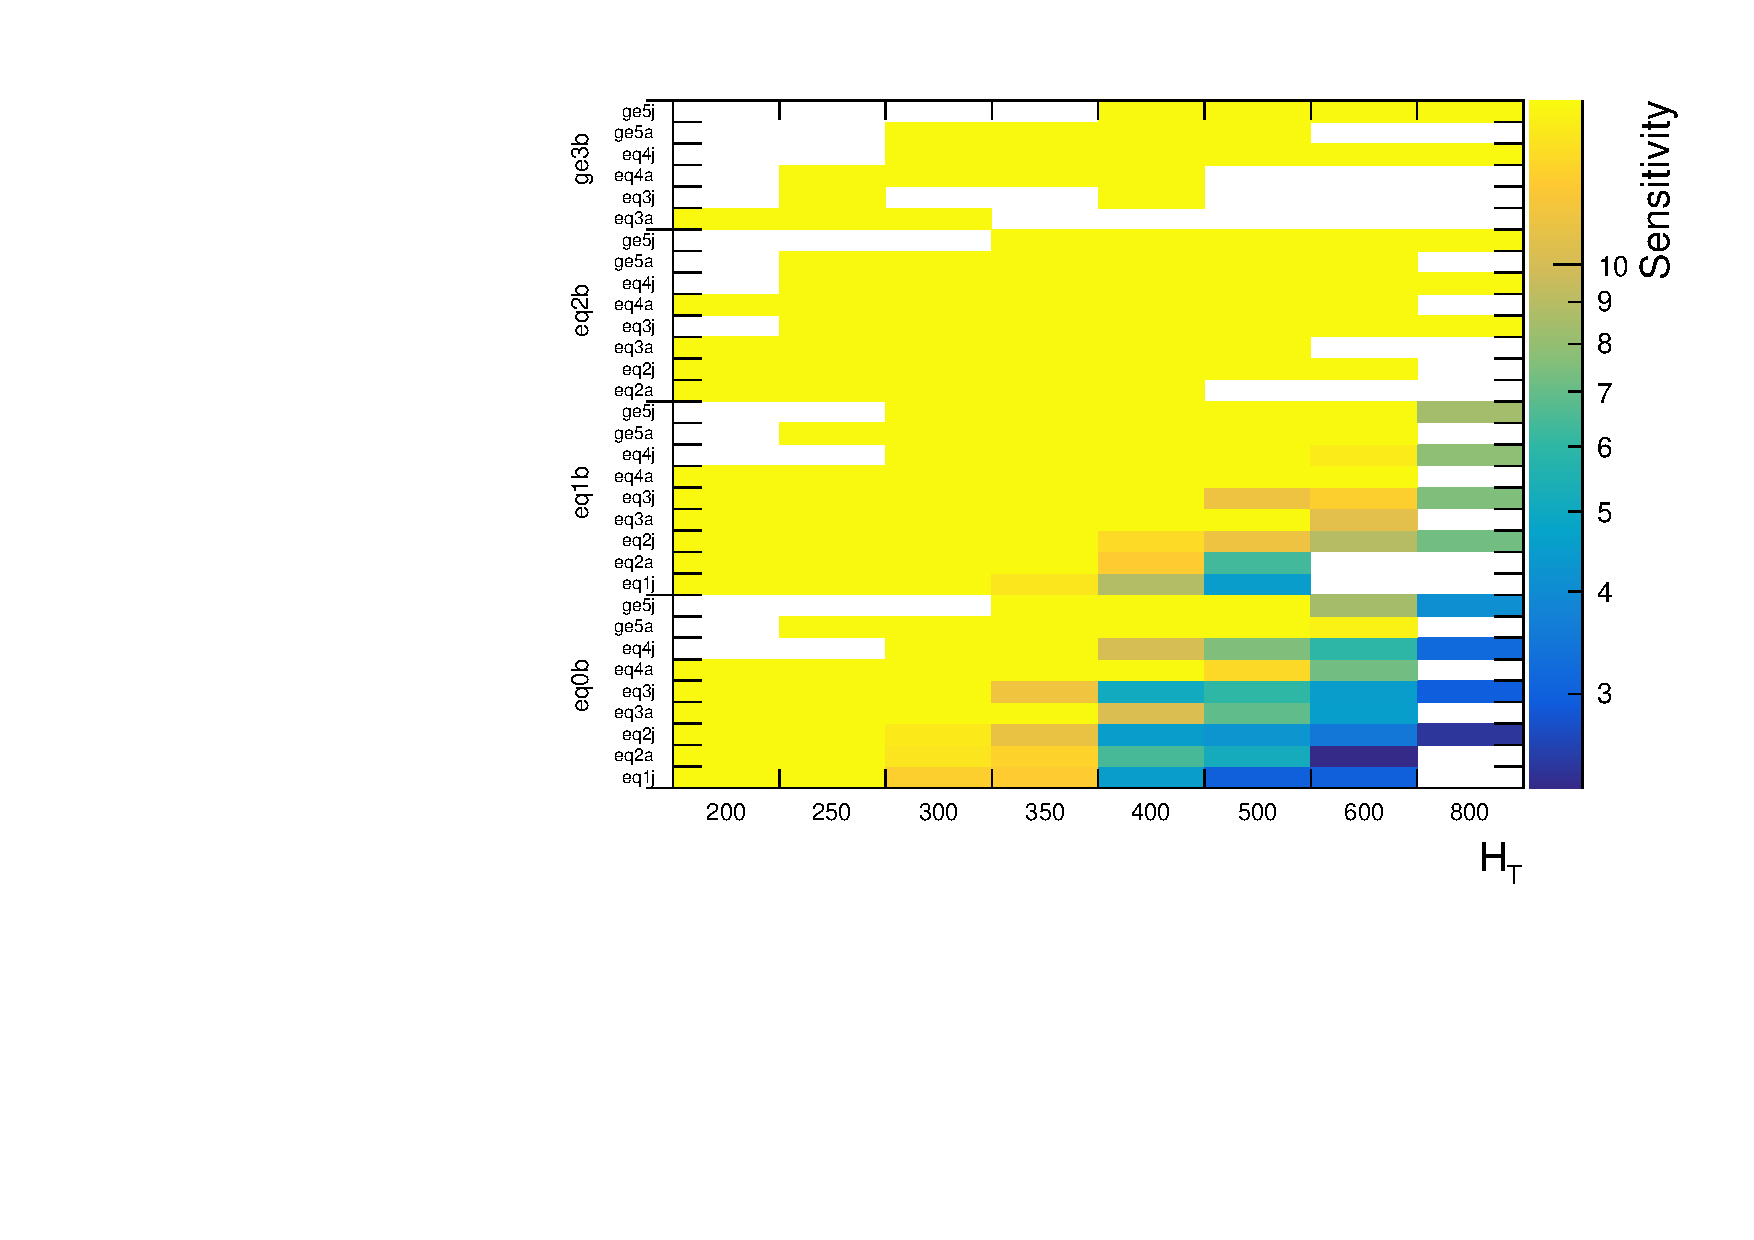
\includegraphics[width=0.5\textwidth]{figures/DMplots/DMA-1500-50_limitPerBin_exp_log}}
\subfigure[Axial vector Mmed=1250 GeV, mDM=350 GeV]{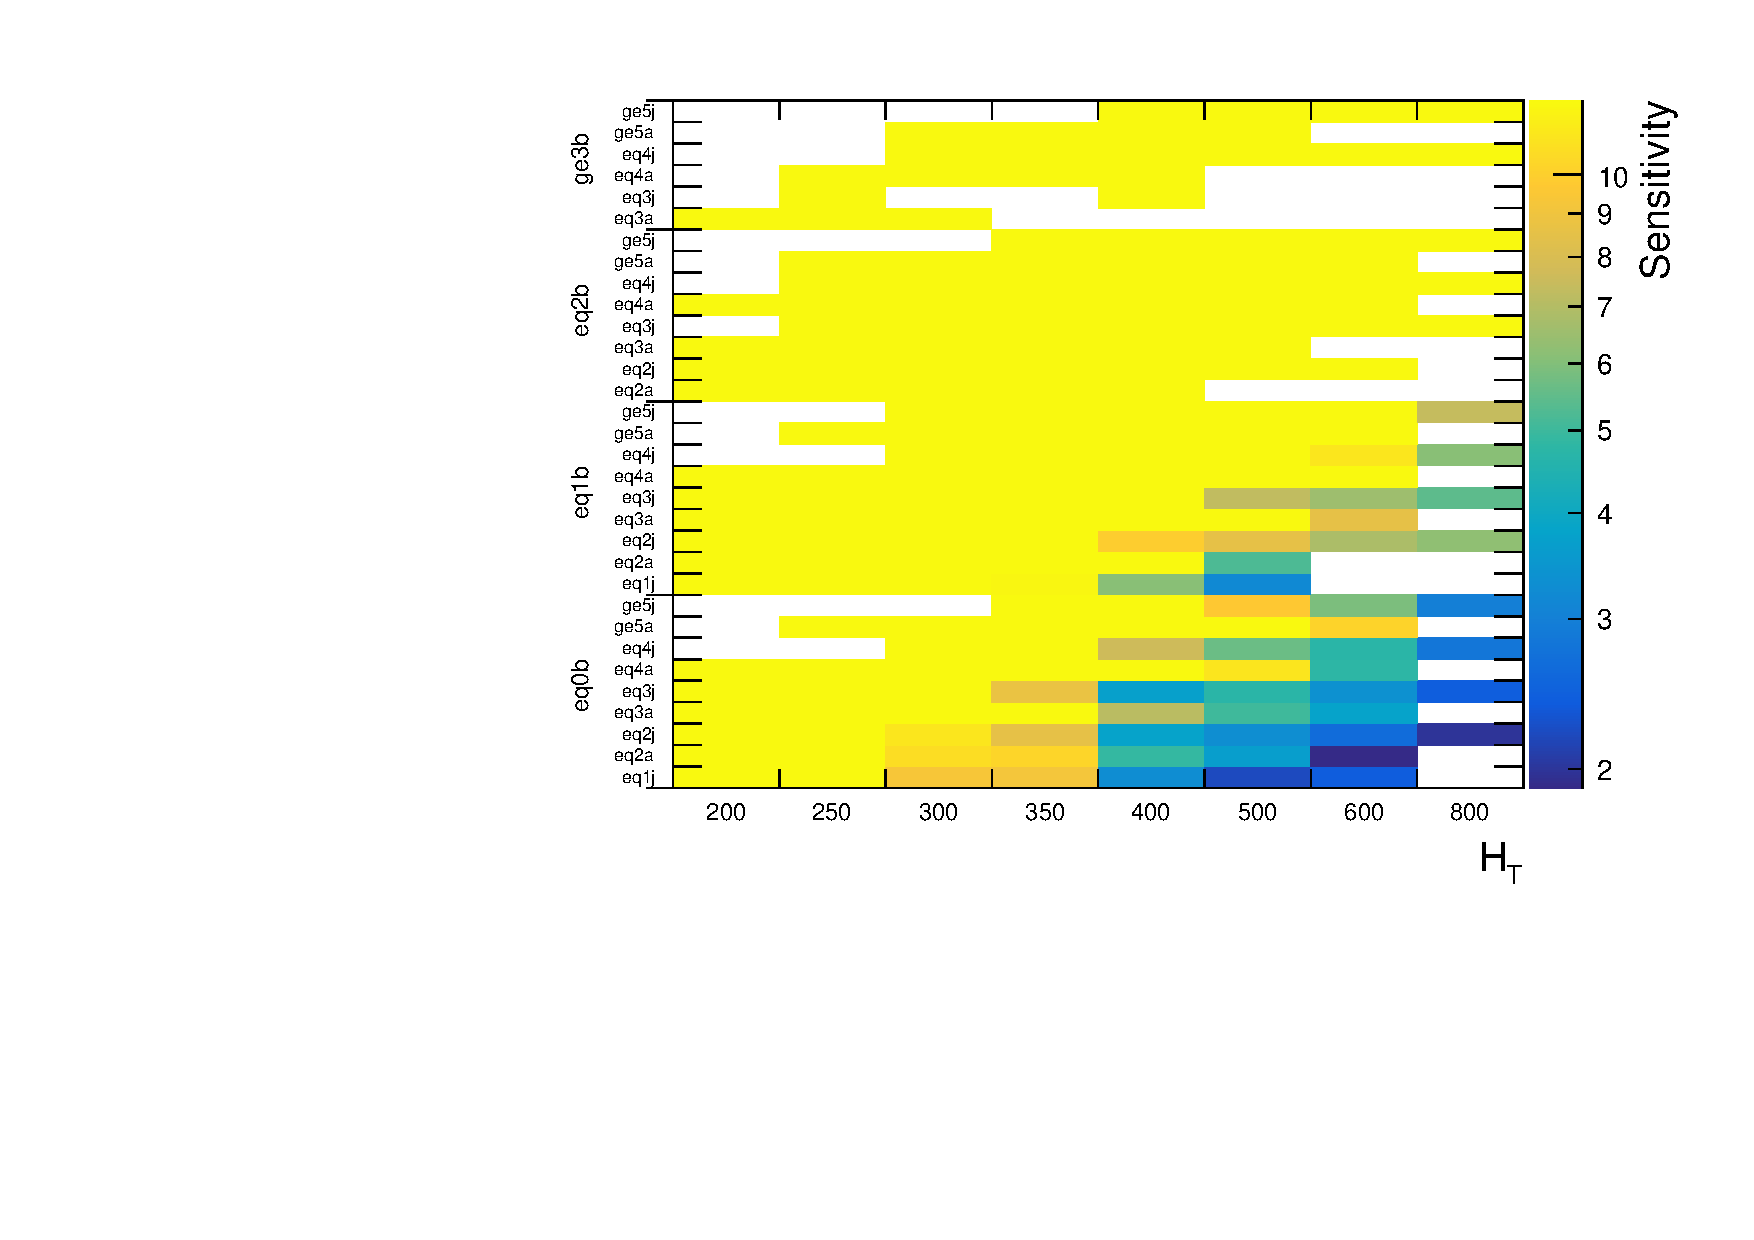
\includegraphics[width=0.5\textwidth]{figures/DMplots/DMA-1250-350_limitPerBin_exp_log}}
\caption{Expected sensitivity from each (\nj,\nb,\scalht) category for the axial vector model.}
\label{fig:DMA-sensitivity} 
\end{figure}

\begin{figure}[h!] \centering
\subfigure[Vector Mmed=1500 GeV, mDM=200 GeV]{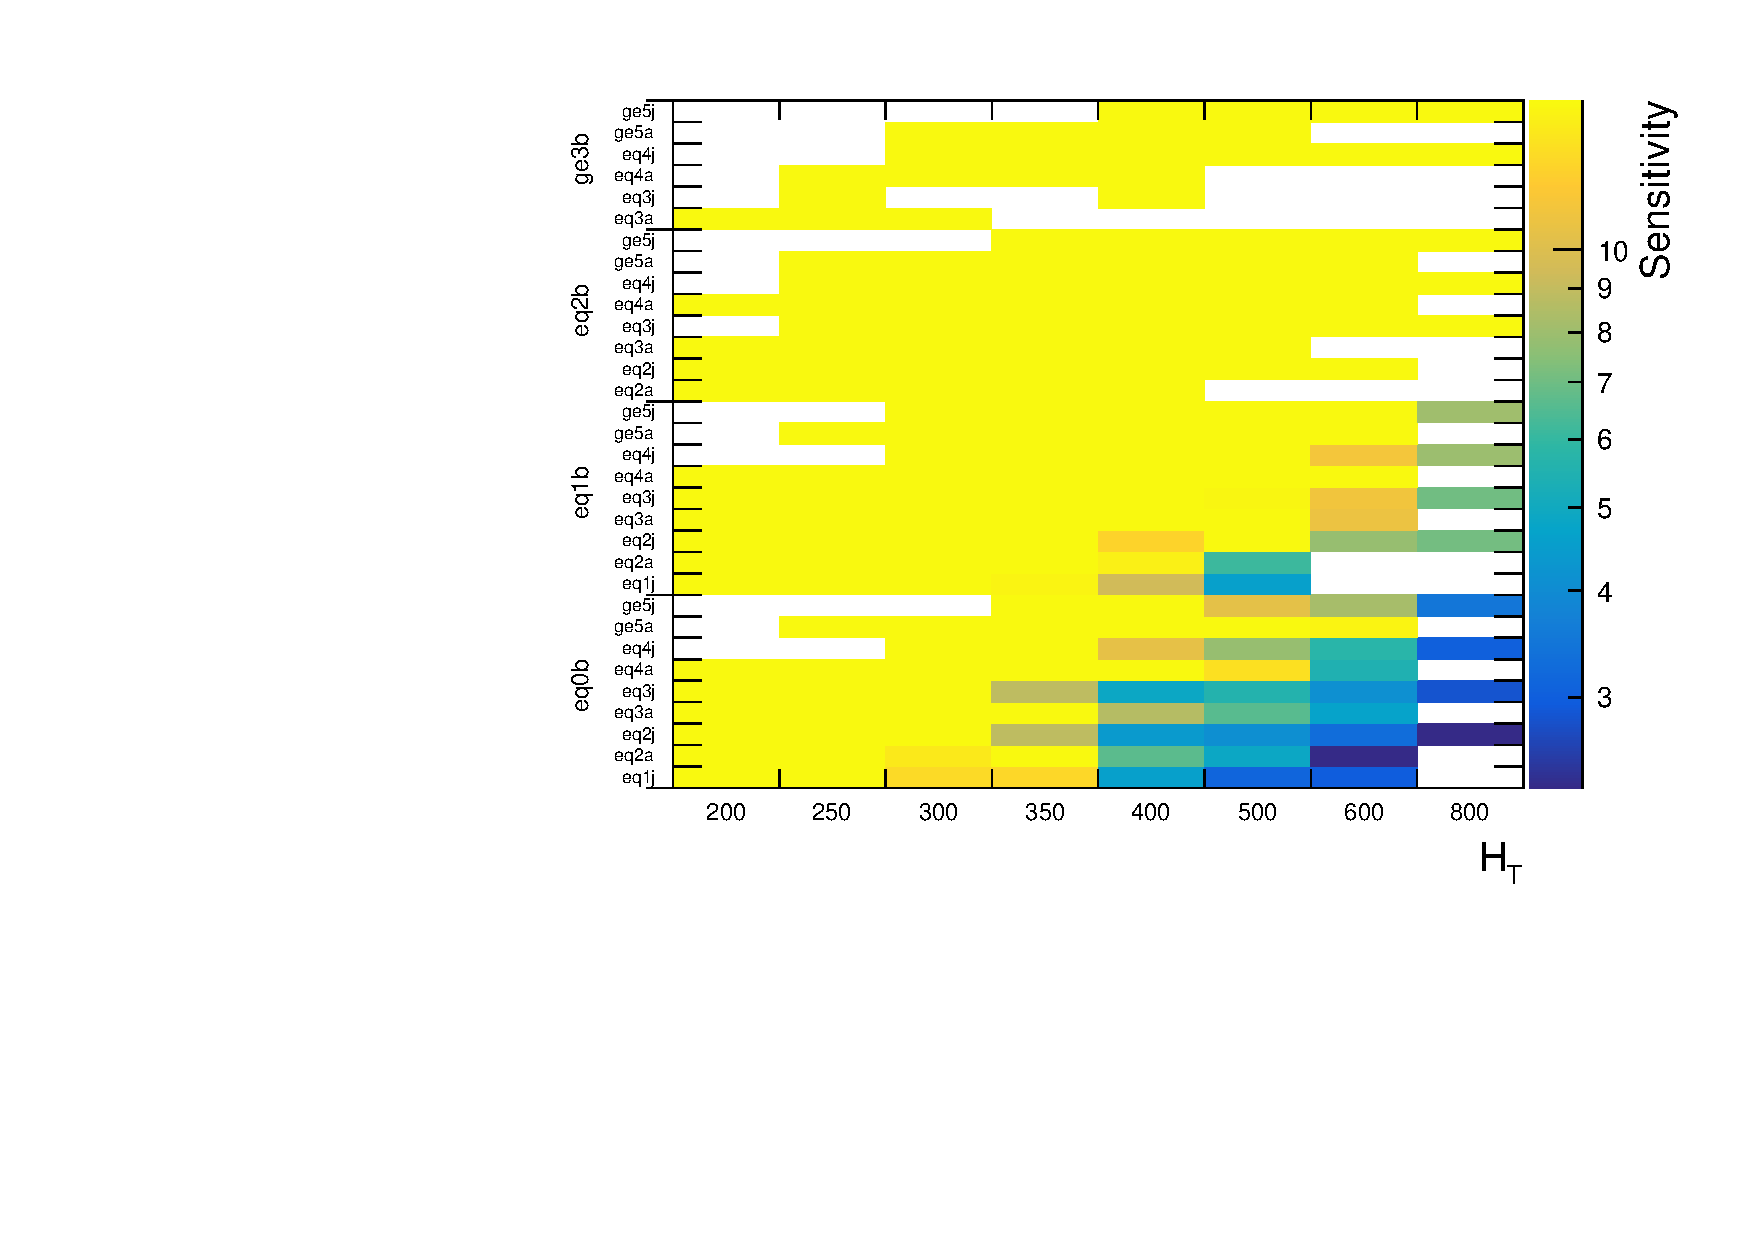
\includegraphics[width=0.5\textwidth]{figures/DMplots/DMV-1500-200_limitPerBin_exp_log}}
\subfigure[Vector Mmed=1250 GeV, mDM=400 GeV]{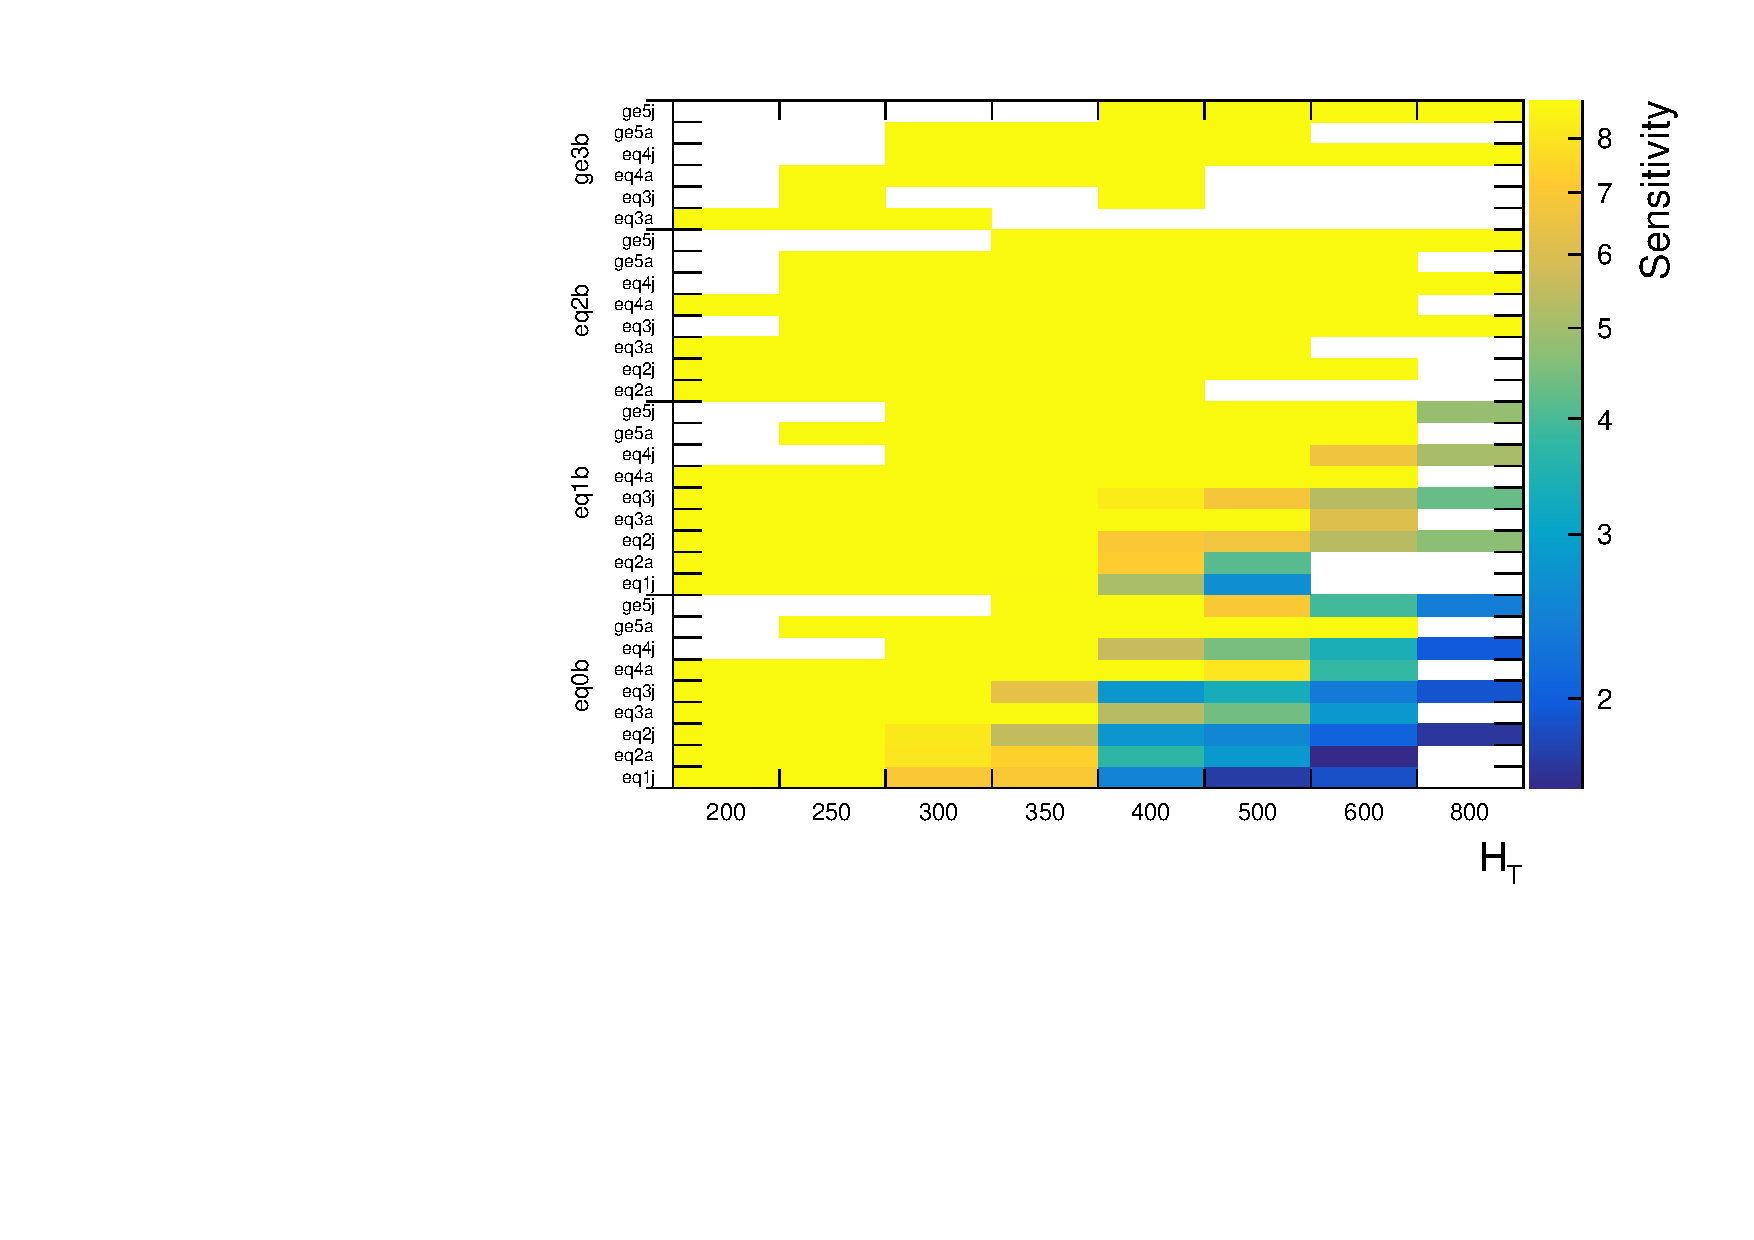
\includegraphics[width=0.5\textwidth]{figures/DMplots/DMV-1250-400_limitPerBin_exp_log}}
\caption{Expected sensitivity from each (\nj,\nb,\scalht) category for the vector model.}
\label{fig:DMV-sensitivity} 
\end{figure}

\begin{figure}[h!] \centering
\subfigure[Pseudoscalar - DMtt Mmed=20 GeV, mDM=1 GeV]{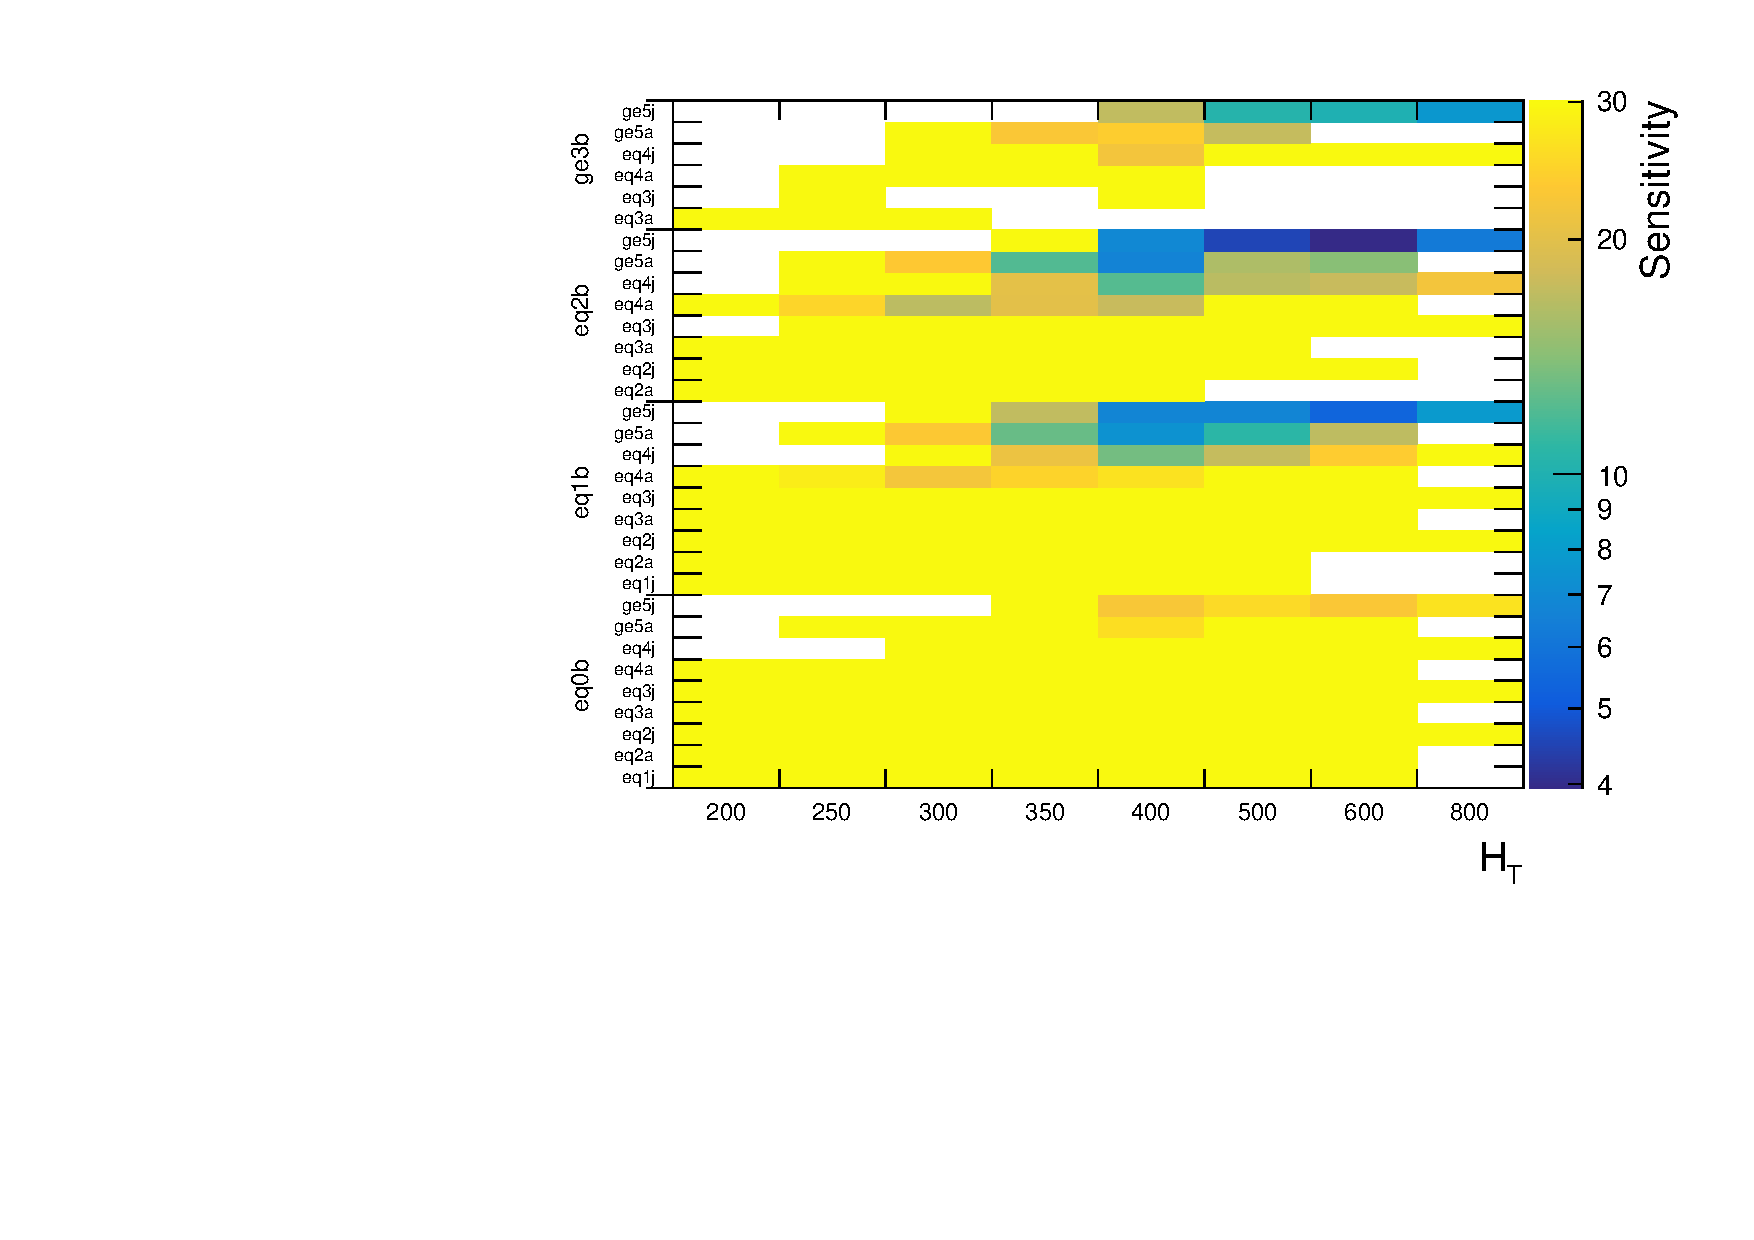
\includegraphics[width=0.5\textwidth]{figures/DMplots/DMttP-20-1_limitPerBin_exp_log}}
\subfigure[Pseudoscalar - DMtt Mmed=100 GeV, mDM=10 GeV]{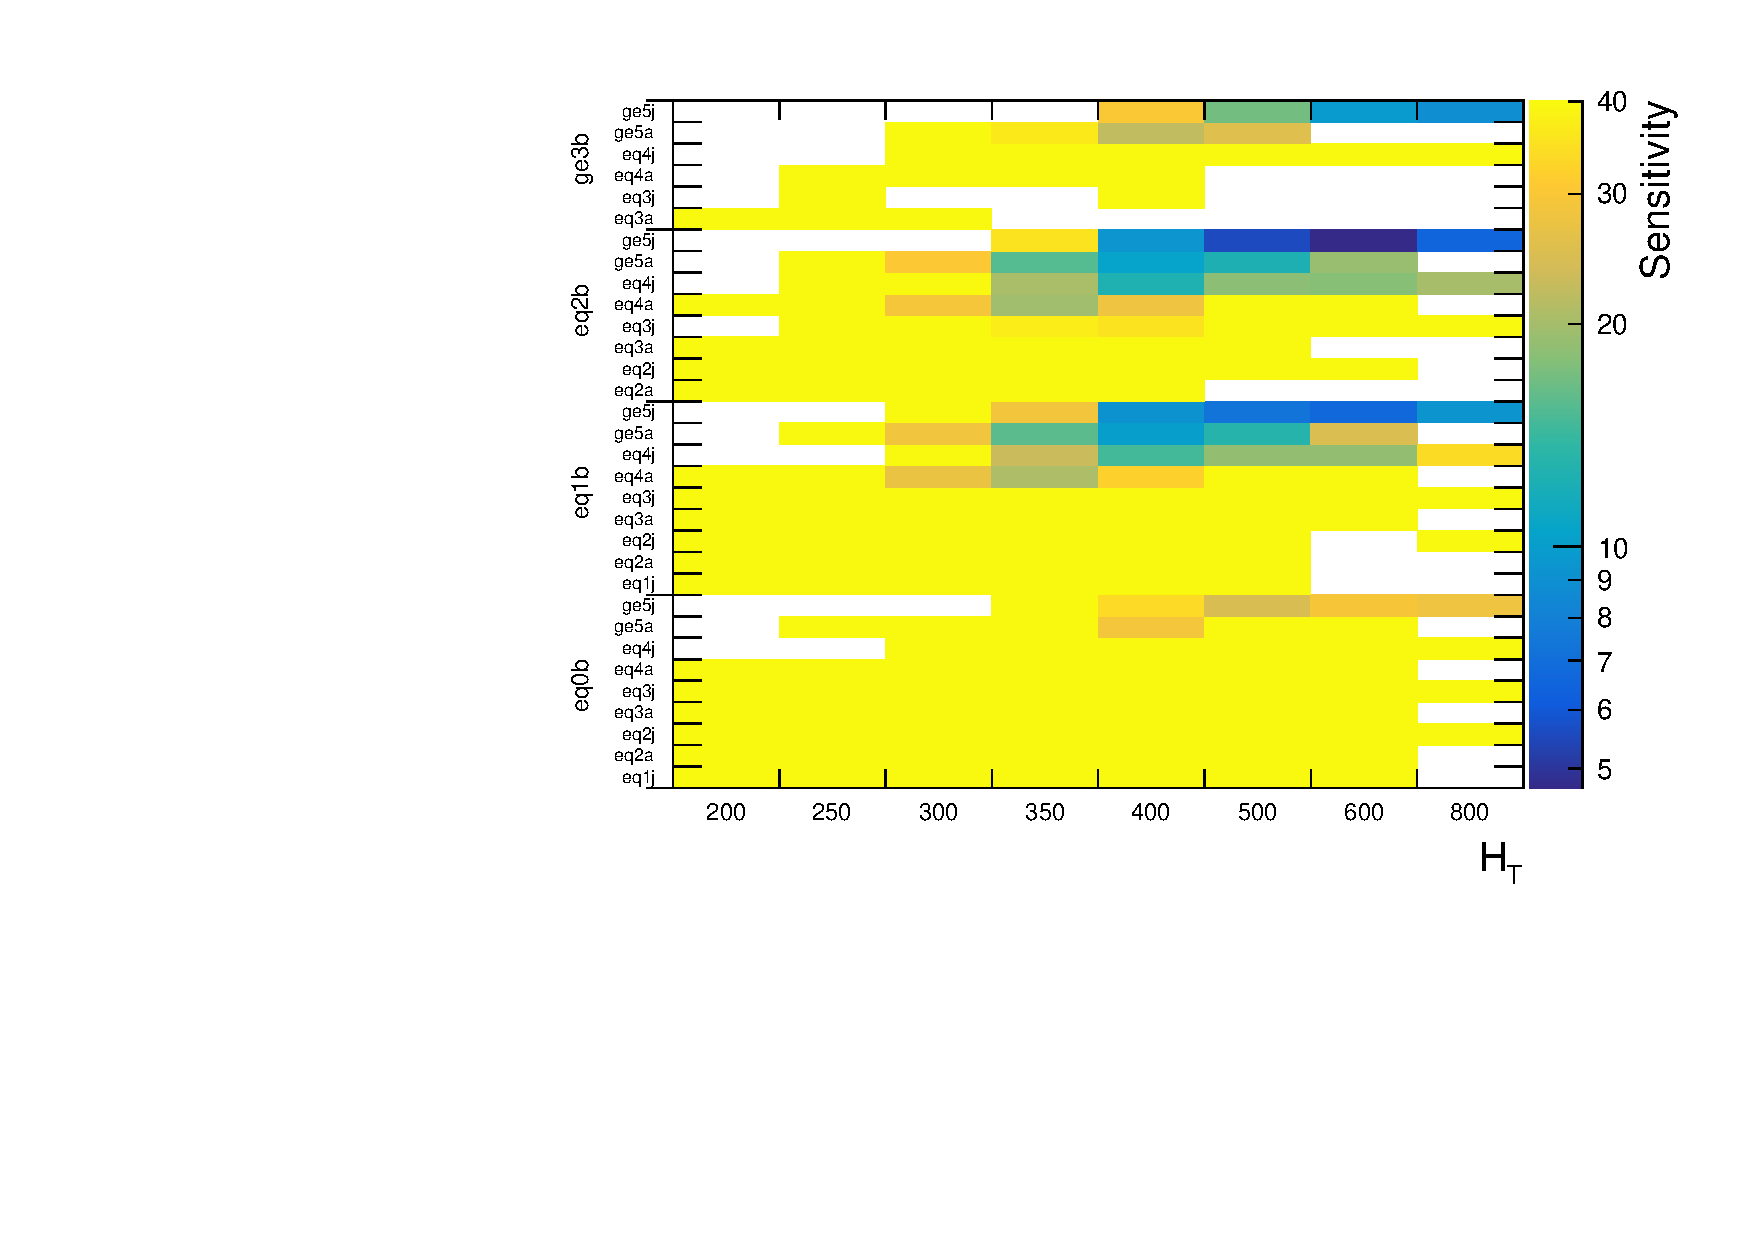
\includegraphics[width=0.5\textwidth]{figures/DMplots/DMttP-100-10_limitPerBin_exp_log}}
\caption{Expected sensitivity from each (\nj,\nb,\scalht) category for the pseudoscalar DMtt model.}
\label{fig:DMttP-sensitivity} 
\end{figure}

\begin{figure}[h!] \centering
\subfigure[Scalar - DMtt Mmed=20 GeV, mDM=1 GeV]{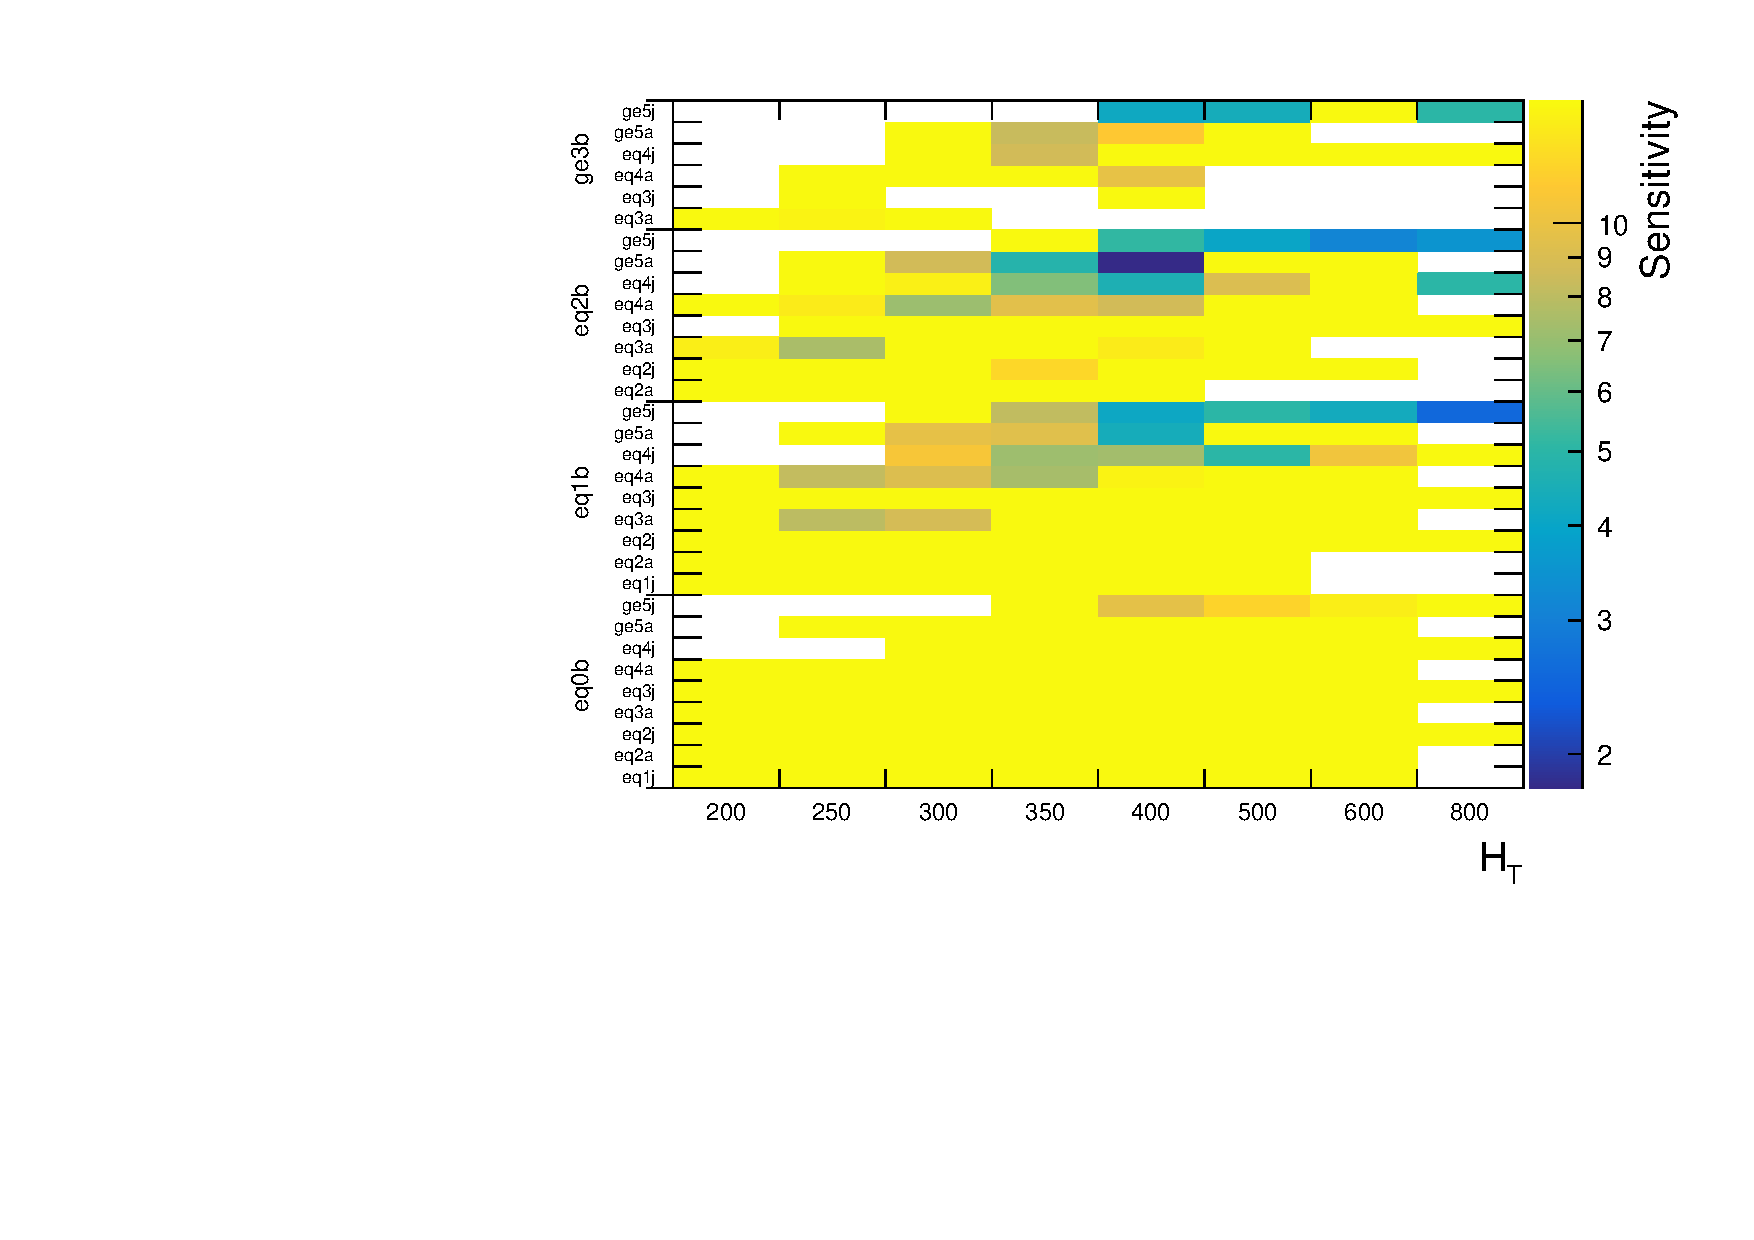
\includegraphics[width=0.5\textwidth]{figures/DMplots/DMttS-20-1_limitPerBin_exp_log}}
\subfigure[Scalar - DMtt Mmed=50 GeV, mDM=10 GeV]{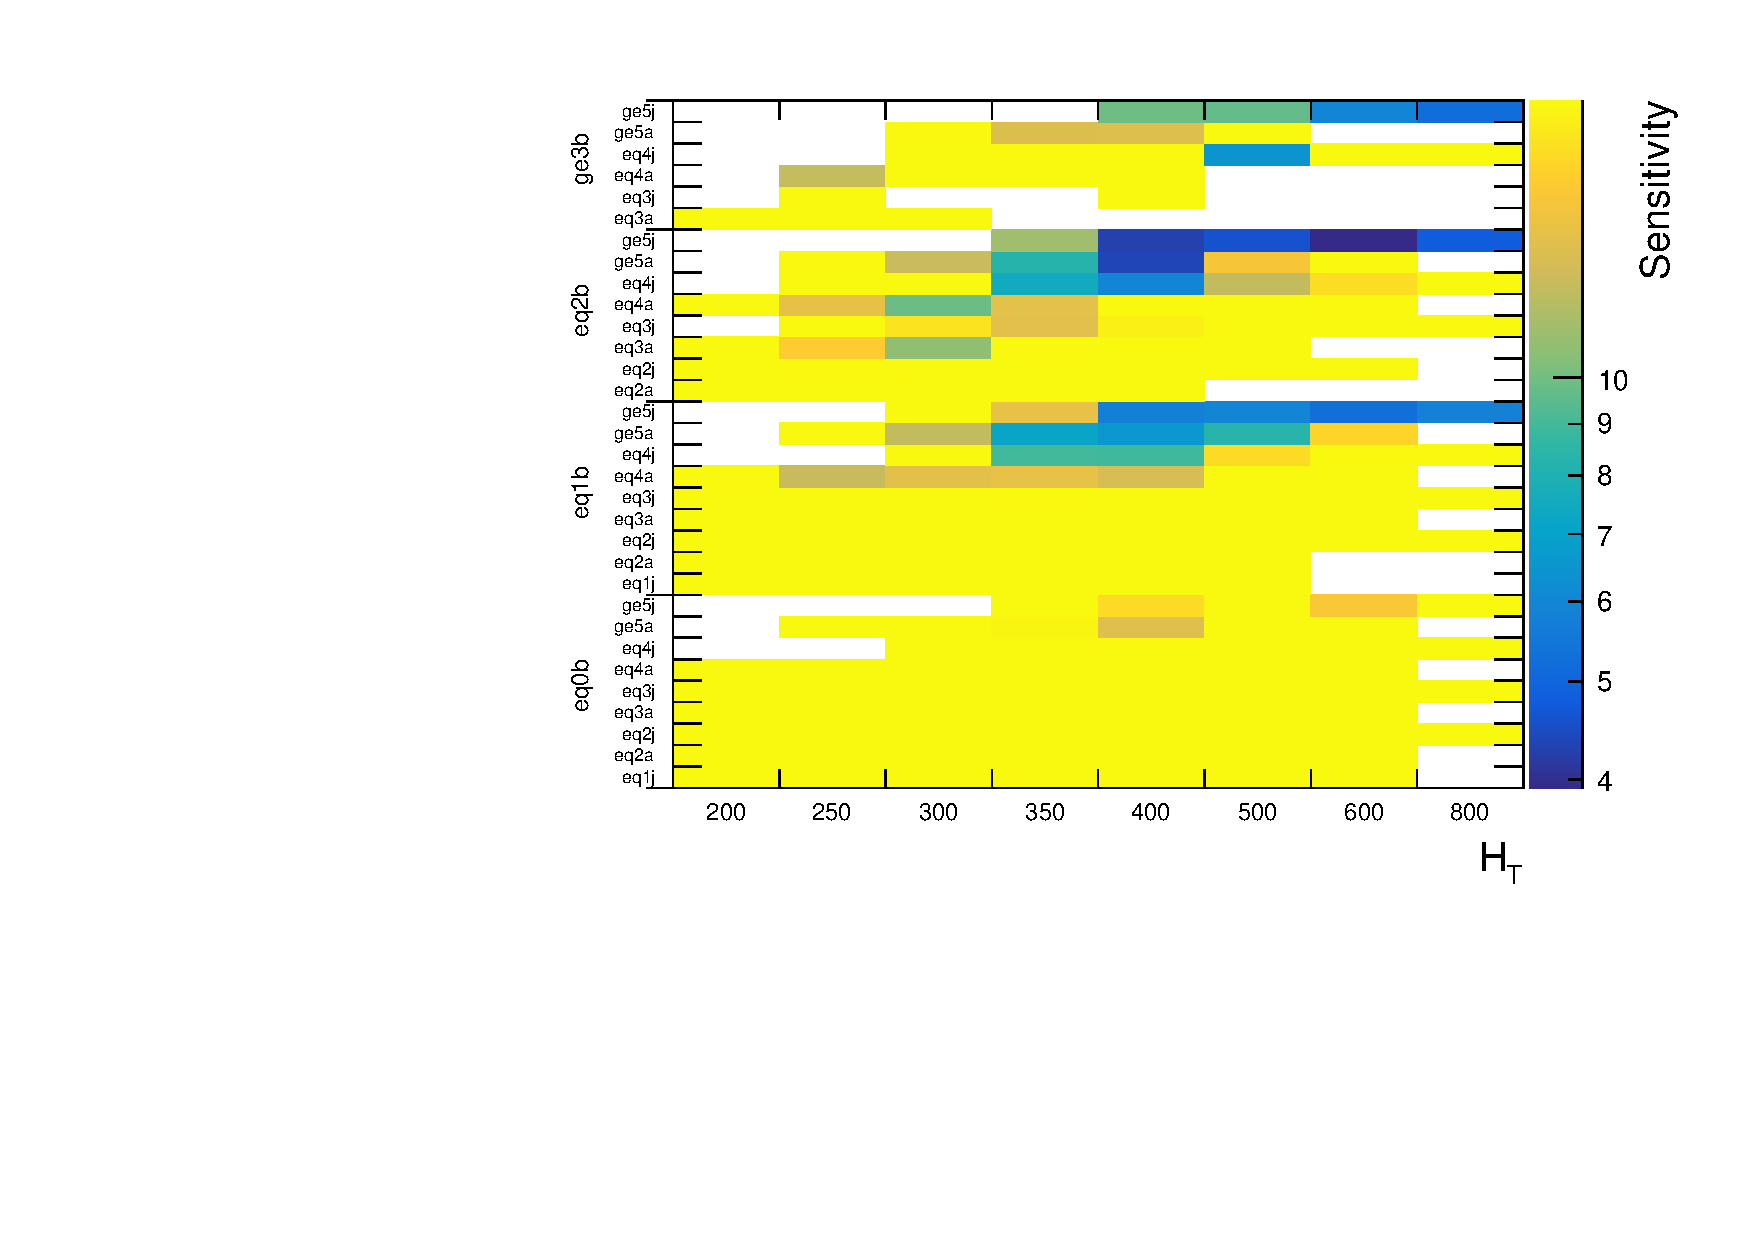
\includegraphics[width=0.5\textwidth]{figures/DMplots/DMttS-50-10_limitPerBin_exp_log}}
\caption{Expected sensitivity from each (\nj,\nb,\scalht) category for the scalar DMtt model.}
\label{fig:DMttS-sensitivity} 
\end{figure}


\clearpage
\subsection{Exclusion limits}
In order to extract the signal contribution in the fit, the distribution of
events according to the \mht variable, encoded as template histograms, is used
as described in Sec.~\ref{sec:had-shape} and \ref{sec:likelihood}. Upper limits
on the cross section are computed using the $\text{CL}_{s}$ criterion 
\cite{CLsTechnique}. Asymptotic formulae \cite{AsymptoticFormulae} are utilised
to approximate the distribution of the test statistics. All the statistical
results are produced using the \textit{combine} tool, provided within the
HiggsAnalysis-CombinedLimit package \cite{Combine}.

In Tab. ~\ref{tab:DMV_limits}-\ref{tab:DMttPS_limits} the 95\% C.L. upper limits 
on the cross section are listed for the models considered in this 
interpretation. These results correspond to 12.9~\ifb of integrated luminosity. 

\begin{table}[!htbp]
  \centering
    \begin{tabular}{rrcc}
        \hline\hline
        \mphi & \mchi & exp r-value & obs r-value \\
        \hline
        500 & 200 & $0.088_{-0.025}^{+0.036}$ & 0.12 \\
        300 & 150 & $0.233_{-0.066}^{+0.094}$ & 0.445 \\
        1000 & 350 & $0.323_{-0.091}^{+0.133}$ & 0.239 \\
        1250 & 150 & $0.56_{-0.16}^{+0.23}$ & 0.318 \\
        1250 &   1 & $0.56_{-0.16}^{+0.23}$ & 0.398 \\
        1250 & 350 & $0.57_{-0.16}^{+0.24}$ & 0.4 \\
        1250 & 250 & $0.57_{-0.16}^{+0.24}$ & 0.412 \\
        1250 & 400 & $0.62_{-0.17}^{+0.25}$ & 0.43 \\
        1500 & 200 & $0.96_{-0.27}^{+0.39}$ & 0.73 \\
        1500 &  50 & $1.00_{-0.28}^{+0.42}$ & 0.717 \\
        1500 & 150 & $1.01_{-0.29}^{+0.42}$ & 0.658 \\
        1500 & 100 & $1.03_{-0.29}^{+0.43}$ & 0.663 \\
        \hline\hline
    \end{tabular}
    \caption{Expected and observed limits for vector mediated DM+jets models}
    \label{tab:DMV_limits}
\end{table}

\begin{table}[]
    \centering
    \begin{tabular}{rrcc}
        \hline\hline
        \mphi & \mchi & exp r-value & obs r-value \\
        \hline
          300 &   1 & $0.038_{-0.011}^{+0.015}$ & 0.0848 \\
          300 & 100 & $0.062_{-0.017}^{+0.026}$ & 0.137 \\
          500 &   1 & $0.071_{-0.020}^{+0.028}$ & 0.074 \\
          500 & 150 & $0.112_{-0.031}^{+0.046}$ & 0.143 \\
          500 & 200 & $0.198_{-0.056}^{+0.081}$ & 0.258 \\
         1000 & 300 & $0.46_{-0.13}^{+0.19}$ & 0.325 \\
         1250 &  10 & $0.54_{-0.15}^{+0.23}$ & 0.337 \\
         1250 & 100 & $0.56_{-0.16}^{+0.23}$ & 0.381 \\
         1000 & 350 & $0.58_{-0.16}^{+0.24}$ & 0.569 \\
         1250 & 150 & $0.58_{-0.16}^{+0.24}$ & 0.406 \\
         1250 & 200 & $0.60_{-0.17}^{+0.25}$ & 0.407 \\
         1250 & 250 & $0.64_{-0.18}^{+0.27}$ & 0.512 \\
         1250 & 300 & $0.71_{-0.20}^{+0.30}$ & 0.491 \\
         1250 & 350 & $0.79_{-0.22}^{+0.32}$ & 0.527 \\
         1500 & 150 & $0.99_{-0.28}^{+0.42}$ & 0.579 \\
         1500 &  50 & $1.00_{-0.28}^{+0.41}$ & 0.609 \\
         1500 & 100 & $1.03_{-0.29}^{+0.43}$ & 0.66 \\
         1500 & 200 & $1.08_{-0.31}^{+0.45}$ & 0.689 \\
         1500 & 250 & $1.12_{-0.32}^{+0.47}$ & 0.784 \\
         1500 & 300 & $1.16_{-0.33}^{+0.48}$ & 0.743 \\
         1500 & 350 & $1.23_{-0.35}^{+0.52}$ & 0.767 \\
         1500 & 400 & $1.35_{-0.39}^{+0.56}$ & 0.819 \\
        \hline\hline
    \end{tabular}
    \caption{Expected and observed limits for axial-vector mediated DM+jets models}
    \label{tab:DMAV_limits}
\end{table}

%\begin{table}[]
%  \centering
%  \begin{tabular}{rrcccc}
%    \hline\hline
%    $M_{\text{med}}$ & $M_{\text{DM}}$ & nJet MSB & exp r-value\\
%    \hline
%%%% 12.9 /fb
%      300 &   1 & eq4a, eq3a, eq1j, eq3j & $1.73_{-0.53}^{+0.82}$     \\ %& 1.94 \\
%       10 &   1 & eq2j, eq3j, eq4j, eq3a & $2.36_{-0.67}^{+0.94}$     \\ %& 6.03 \\
%      100 &   1 & eq3j, eq2j, eq3a, eq4j & $2.65_{-0.75}^{+1.07}$     \\ %& 7.97 \\
%      300 & 100 & eq3j, eq2j, eq4j, ge5j & $3.27_{-0.93}^{+1.31}$     \\ %& 9.19 \\
%      500 &   1 & eq3j, eq2j, ge5j, eq4j & $5.8_{-1.6}^{+2.4}$        \\ %& 13.4 \\
%      500 & 150 & eq3j, eq2j, ge5j, eq4j & $7.6_{-2.2}^{+3.1}$        \\ %& 19.4 \\
%     %1000 &   1 & eq3j, ge5j, eq2j, eq4j & $57_{-16}^{+23}$           \\ %& 59.7 \\
%      100 &  50 & eq3j, eq2j, ge5j, eq3a & $62_{-18}^{+25}$           \\ %& 236.0 \\
%     %1250 &  50 & eq4j, eq3j, ge5j, eq2j & $149_{-42}^{+61}$          \\ %& 119.0 \\
%     %1250 &   1 & eq3j, ge5j, eq4j, eq2j & $149_{-42}^{+61}$          \\ %& 122.0 \\
%     %1250 &  10 & eq3j, eq4j, ge5j, eq2j & $154_{-44}^{+62}$          \\ %& 113.0 \\
%     %1250 & 200 & eq3j, eq4j, ge5j, eq2j & $170_{-48}^{+70}$          \\ %& 141.0 \\
%     %1250 & 250 & eq3j, eq4j, ge5j, eq2j & $186_{-53}^{+76}$          \\ %& 135.0 \\
%     %1250 & 300 & ge5j, eq3j, eq4j, eq2j & $199_{-57}^{+82}$          \\ %& 165.0 \\
%     %1250 & 350 & eq3j, ge5j, eq4j, eq2j & $232_{-66}^{+95}$          \\ %& 190.0 \\
%     %1250 & 400 & ge5j, eq3j, eq4j, eq2j & $278_{-79}^{+113}$         \\ %& 219.0 \\
%     %1500 &  10 & eq3j, ge5j, eq4j, eq2j & $357.2_{-101.4}^{+146.7}$  \\ %& 271.0 \\
%     %1500 &  50 & eq4j, ge5j, eq3j, eq2j & $359.2_{-102.0}^{+147.5}$  \\ %& 253.0 \\
%     %1500 &   1 & eq3j, eq4j, ge5j, eq2j & $365.2_{-103.7}^{+150.0}$  \\ %& 249.0 \\
%     %1500 & 100 & ge5j, eq3j, eq4j, eq2j & $367.8_{-104.4}^{+151.0}$  \\ %& 280.0 \\
%     %1500 & 200 & ge5j, eq3j, eq4j, eq2j & $399.2_{-113.3}^{+163.9}$  \\ %& 327.0 \\
%     %1500 & 250 & eq4j, ge5j, eq3j, eq2j & $423.9_{-120.3}^{+174.0}$  \\ %& 293.0 \\
%     %1500 & 300 & ge5j, eq4j, eq3j, eq2j & $453.2_{-128.7}^{+186.1}$  \\ %& 305.0 \\
%     %1500 & 350 & eq3j, eq4j, ge5j, eq2j & $497.2_{-141.2}^{+204.2}$  \\ %& 301.0 \\
%     %1500 & 400 & eq3j, ge5j, eq4j, eq2j & $537.0_{-152.4}^{+220.5}$  \\ %& 356.0 \\
%     %2000 &   1 & eq4j, ge5j, ge5a, eq1j & $2339.8_{-669.8}^{+960.6}$ \\ %& 1720.0 \\
%    \hline\hline
%  \end{tabular}
%  \caption{Expected limits for scalar mediated DM+jets models}
%  \label{tab:DMS_limits}
%\end{table}

%\begin{table}[]
%  \centering
%  \begin{tabular}{rrcccc}
%    \hline\hline
%    $M_{\text{med}}$ & $M_{\text{DM}}$ & nJet MSB & exp r-value\\
%    \hline
%%%% 12.9 /fb
%       10 &   1 & eq2j, eq3j, eq3a, eq4j & $1.03_{-0.29}^{+0.41}$ \\ %& 2.88 \\
%      300 &   1 & eq3j, eq2j, ge5j, eq4j & $1.13_{-0.32}^{+0.45}$ \\ %& 3.31 \\
%      300 & 100 & eq3j, eq2j, eq4j, ge5j & $1.14_{-0.32}^{+0.46}$ \\ %& 2.81 \\
%      100 &   1 & eq3j, eq2j, ge5j, eq4j & $1.18_{-0.33}^{+0.47}$ \\ %& 4.2 \\
%      500 &   1 & eq3j, eq2j, ge5j, eq4j & $3.42_{-0.96}^{+1.40}$ \\ %& 7.5 \\
%      500 & 150 & eq3j, eq2j, eq4j, ge5j & $3.8_{-1.1}^{+1.5}$    \\ %& 8.82 \\
%      500 & 200 & eq3j, eq2j, ge5j, eq4j & $4.6_{-1.3}^{+1.9}$    \\ %& 9.72 \\
%      300 & 150 & eq3j, eq2j, ge5j, eq4j & $9.3_{-2.6}^{+3.8}$    \\ %& 26.6 \\
%      100 &  50 & eq3j, eq2j, ge5j, eq4j & $12.4_{-3.5}^{+5.0}$   \\ %& 32.9 \\
%       10 &  10 & eq3j, eq2j, ge5j, eq3a & $14.4_{-4.1}^{+5.8}$   \\ %& 36.8 \\
%     %1000 & 300 & eq3j, eq4j, ge5j, eq2j & $51_{-15}^{+21}$       \\ %& 41.4 \\
%     %1000 & 350 & eq3j, eq4j, ge5j, eq2j & $57_{-16}^{+23}$       \\ %& 60.5 \\
%     %1250 &   1 & eq3j, ge5j, eq2j, eq4j & $114_{-32}^{+47}$      \\ %& 84.1 \\
%     %1250 & 100 & eq3j, eq4j, ge5j, eq2j & $116_{-33}^{+47}$      \\ %& 85.2 \\
%     %1250 & 150 & eq3j, eq4j, ge5j, eq2j & $118_{-34}^{+48}$      \\ %& 96.4 \\
%     %1250 & 200 & eq3j, eq4j, ge5j, eq2j & $122_{-35}^{+50}$      \\ %& 104.0 \\
%     %1250 & 250 & ge5j, eq3j, eq4j, eq2j & $125_{-36}^{+51}$      \\ %& 112.0 \\
%     %1250 & 300 & eq3j, eq4j, ge5j, eq2j & $132_{-38}^{+53}$      \\ %& 95.4 \\
%     %1250 & 350 & eq3j, eq4j, ge5j, eq2j & $137_{-39}^{+56}$      \\ %& 107.0 \\
%     %1250 & 400 & eq3j, eq4j, eq2j, ge5j & $147_{-42}^{+60}$      \\ %& 113.0 \\
%     %1500 & 100 & eq3j, ge5j, eq4j, eq2j & $275_{-78}^{+113}$     \\ %& 188.0 \\
%     %1500 &  50 & eq3j, ge5j, eq4j, eq2j & $276_{-78}^{+113}$     \\ %& 188.0 \\
%     %1500 &   1 & eq3j, eq4j, ge5j, eq2j & $281_{-80}^{+115}$     \\ %& 192.0 \\
%     %1500 & 150 & eq4j, eq3j, ge5j, eq2j & $283_{-80}^{+116}$     \\ %& 176.0 \\
%     %1500 &  10 & eq4j, ge5j, eq3j, eq2j & $286_{-81}^{+117}$     \\ %& 192.0 \\
%     %1500 & 200 & eq3j, eq4j, ge5j, eq2j & $294_{-83}^{+121}$     \\ %& 202.0 \\
%     %1500 & 250 & eq3j, eq4j, ge5j, eq2j & $308_{-88}^{+127}$     \\ %& 272.0 \\
%     %1500 & 300 & ge5j, eq3j, eq4j, eq2j & $316_{-90}^{+130}$     \\ %& 231.0 \\
%     %1500 & 350 & eq3j, ge5j, eq4j, eq2j & $331_{-94}^{+136}$     \\ %& 221.0 \\
%     %1500 & 400 & eq4j, ge5j, eq3j, eq2j & $341_{-97}^{+140}$     \\ %& 239.0 \\
%\hline\hline
%  \end{tabular}
%  \caption{Expected limits for pseudoscalar mediated DM+jets models}
%  \label{tab:DMPS_limits}
%\end{table}

\begin{table}[]
    \centering
    \begin{tabular}{rrcc}
        \hline\hline
        \mphi & \mchi & exp r-value & obs r-value \\
        \hline
           10 &   1 & $0.63_{-0.20}^{+0.34}$ & 0.425 \\
           20 &   1 & $0.76_{-0.24}^{+0.41}$ & 0.367 \\
           50 &  10 & $1.00_{-0.32}^{+0.55}$ & 0.59 \\
           50 &   1 & $1.14_{-0.36}^{+0.62}$ & 0.73 \\
          100 &   1 & $1.52_{-0.49}^{+0.83}$ & 1.1 \\
          100 &  10 & $1.59_{-0.51}^{+0.88}$ & 1.35 \\
          200 &  50 & $2.84_{-0.93}^{+1.59}$ & 3.81 \\
          200 &   1 & $2.84_{-0.93}^{+1.59}$ & 3.46 \\
          300 &  50 & $4.5_{-1.5}^{+2.6}$ & 4.83 \\
          300 &   1 & $4.6_{-1.5}^{+2.7}$ & 6.79 \\
          500 &   1 & $16.4_{-5.6}^{+10.1}$ & 22.0 \\
           15 &  10 & $24.1_{-7.8}^{+13.1}$ & 14.1 \\
           10 &  10 & $27.1_{-8.8}^{+14.4}$ & 25.8 \\
           95 &  50 & $68_{-22}^{+39}$ & 77.3 \\
           50 &  50 & $123_{-41}^{+71}$ & 142.0 \\
           10 &  50 & $138_{-46}^{+80}$ & 150.0 \\
        \hline\hline
    \end{tabular}
    \caption{Expected and observed limits for scalar mediated DM+ttbar models}
    \label{tab:DMttS_limits}
\end{table}

\begin{table}[]
    \centering
    \begin{tabular}{rrcc}
        \hline\hline
        \mphi & \mchi & exp r-value & obs r-value \\
        \hline
           10 &   1 & $1.32_{-0.44}^{+0.77}$ & 1.4 \\
           20 &   1 & $1.33_{-0.44}^{+0.77}$ & 1.35 \\
           50 &  10 & $1.38_{-0.46}^{+0.81}$ & 1.74 \\
           50 &   1 & $1.45_{-0.48}^{+0.84}$ & 1.5 \\
          100 &  10 & $1.60_{-0.54}^{+0.93}$ & 2.34 \\
          100 &   1 & $1.60_{-0.53}^{+0.94}$ & 2.11 \\
          200 &  50 & $2.34_{-0.79}^{+1.40}$ & 3.08 \\
          200 &   1 & $2.35_{-0.80}^{+1.41}$ & 3.22 \\
          300 &  50 & $3.6_{-1.2}^{+2.2}$ & 5.59 \\
          300 &   1 & $3.6_{-1.2}^{+2.2}$ & 4.94 \\
          500 &   1 & $17.4_{-6.2}^{+11.0}$ & 23.3 \\
           15 &  10 & $20.3_{-6.7}^{+12.0}$ & 25.9 \\
           95 &  50 & $23.7_{-8.0}^{+14.0}$ & 27.7 \\
           10 &  10 & $24.0_{-8.1}^{+14.1}$ & 22.7 \\
           50 &  50 & $66_{-22}^{+40}$ & 93.1 \\
           10 &  50 & $78_{-26}^{+48}$ & 131.0 \\
        \hline\hline
    \end{tabular}
    \caption{Expected and observed limits for pseudoscalar mediated DM+ttbar models}
    \label{tab:DMttPS_limits}
\end{table}

%Currently we are scaling the expected sensitivities to 2.2~\ifb of data corresponding to last years dataset to be able to compare.
%The expected 95\% CL signal strength for vector-axial (VA) samples with couplings to the SM of $g_\textrm{SM}=0.25$ and $g_\textrm{DM}=0.25$
%is showin on Fig.~\ref{fig:exp_dmj_av}



%\begin{figure}[h!] \centering
%\subfigure{\includegraphics[width=0.35\textwidth]{figures/DMplots/DMA_76X_ContourLimits.pdf}}
%\caption{Expected sensitivities for 2.2~\ifb for the Axial-Vector light jet DM models}
%\label{fig:exp_dmj_av} \end{figure}




%Owing to the principal of Minimal Flavor Violation (MFV), top and bottom quarks can play important roles in the phenomenology of dark matter. Scalar and
%pseudoscalar models predict not only the `monojet' processes described in Sec.~\ref{sec:dm_smdm} but also the production of dark matter in association
%with top (or bottom) pairs. This results in signatures with relatively large jet multiplicities, in particular for \DMtt production. The \alphat analysis is well 
%suited to searching for such signatures. An example Feynman diagram for the pair production of dark matter particles in association with pairs of heavy quarks is
%shown in Fig.~\ref{fig:feynman_hf}.



%\begin{figure}[h!] \centering
%\subfigure{\includegraphics[width=0.35\textwidth]{figures/DMplots/DMA_76X_ContourLimits.pdf}}
%\caption{Expected sensitivities for 2.2~\ifb for the pseudoscalar DM+$t\bar{t}$ models}
%\label{fig:exp_dmtt_ps} \end{figure}
